% !TEX root = ../../main.tex

\FloatBarrier%
\section{Characterisation}\label{appx:def:chara}

\begin{figure}[!htb]

    \begin{subfigure}{0.25\linewidth}
        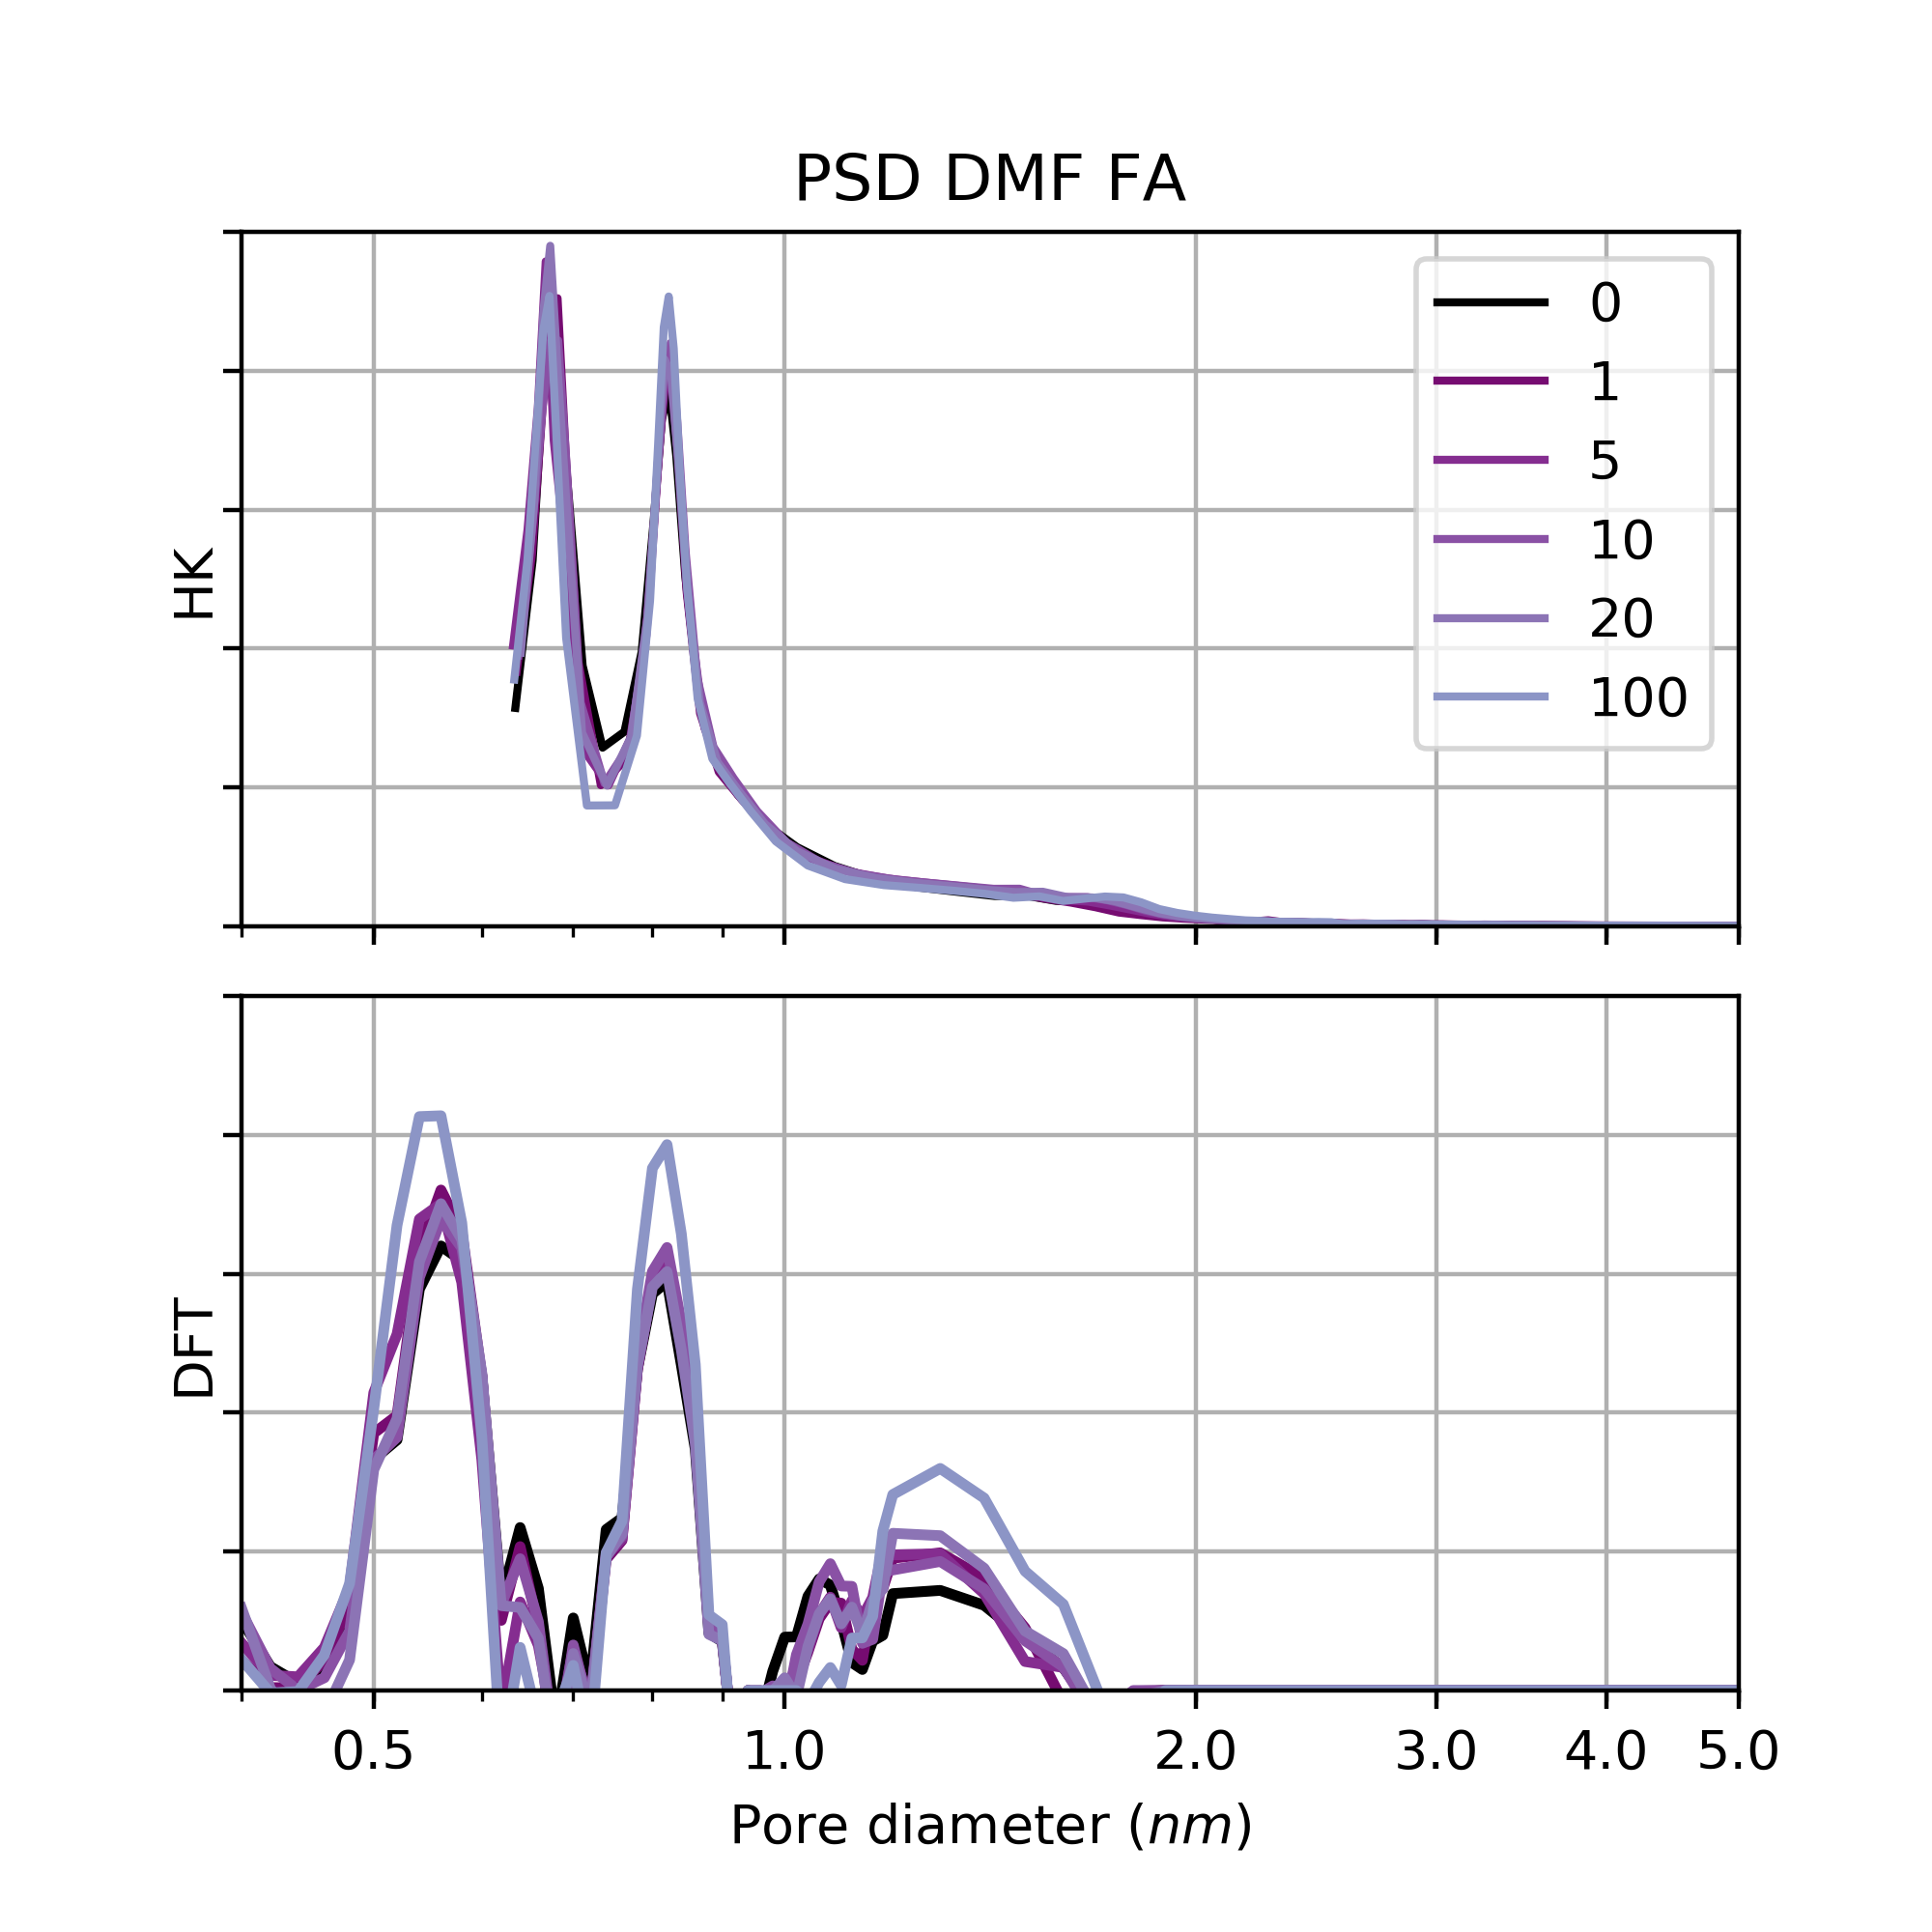
\includegraphics[width=\textwidth]{n2phys/dmf-fa-psd}%
        \label{appx:def:fig:psd-dmf-fa}
    \end{subfigure}%
    \begin{subfigure}{0.25\linewidth}
        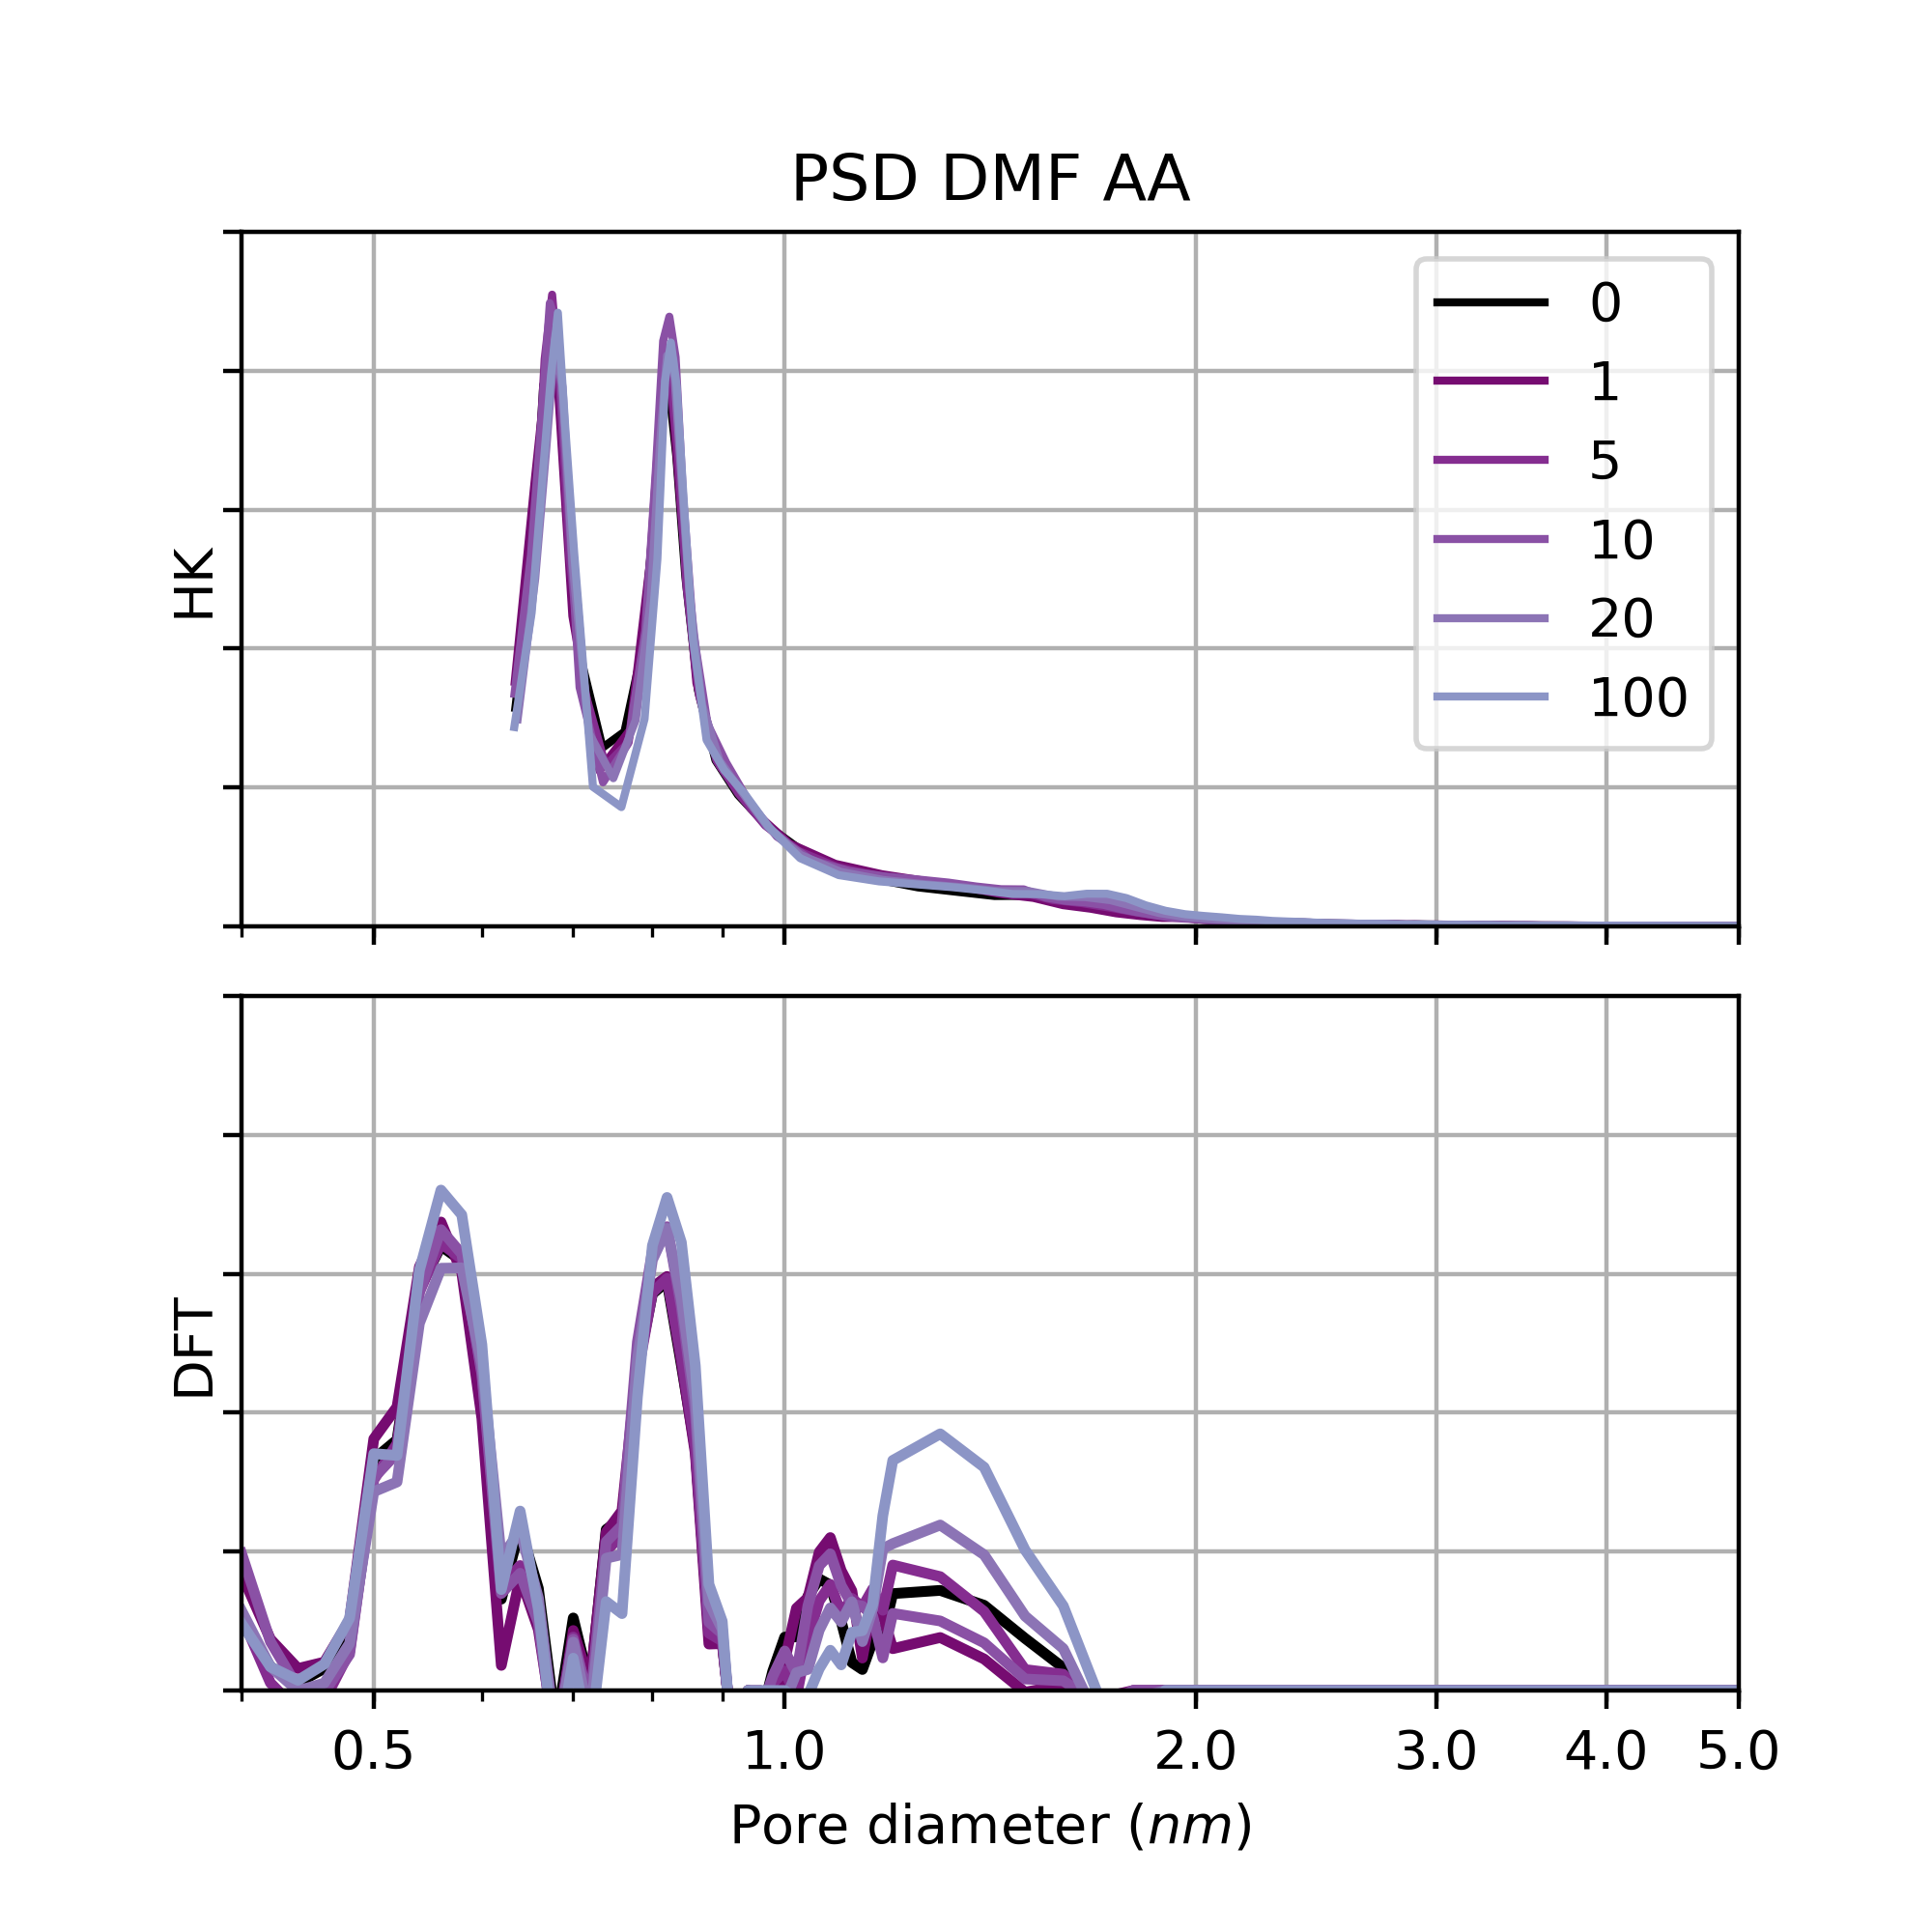
\includegraphics[width=\textwidth]{n2phys/dmf-aa-psd}%
        \label{appx:def:fig:psd-dmf-aa}
    \end{subfigure}%
    \begin{subfigure}{0.25\linewidth}
        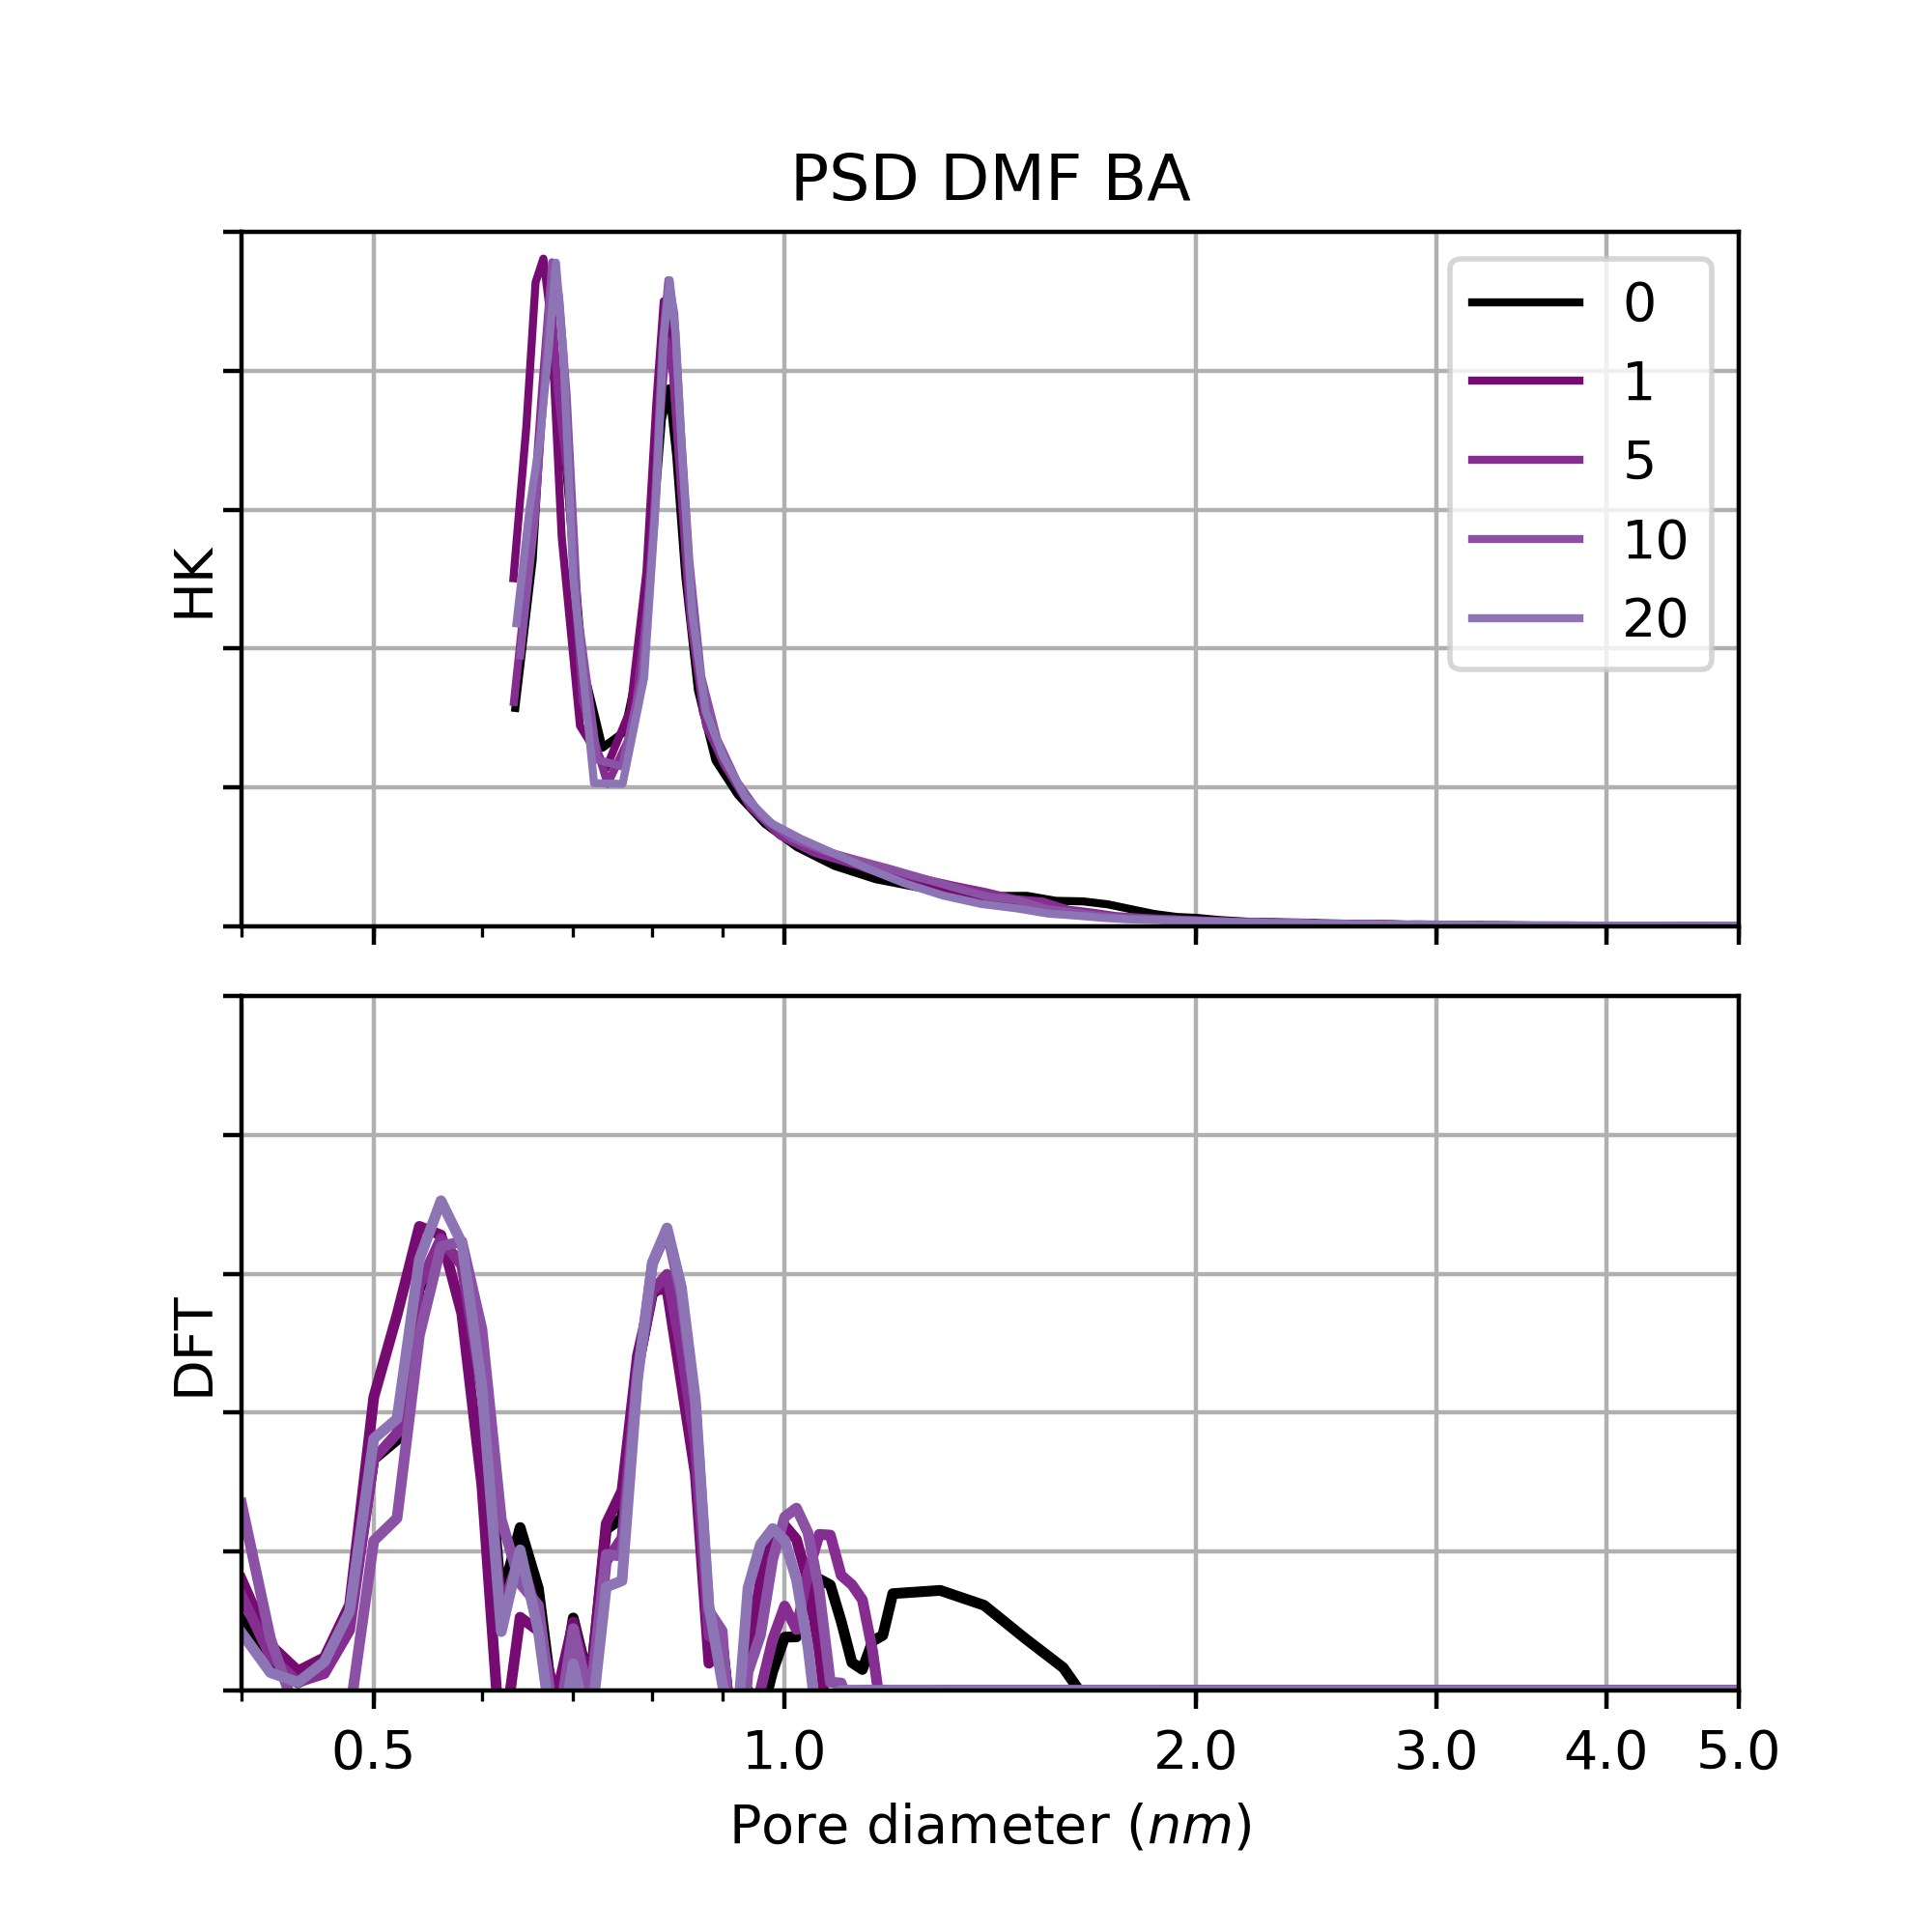
\includegraphics[width=\textwidth]{n2phys/dmf-ba-psd}%
        \label{appx:def:fig:psd-dmf-ba}
    \end{subfigure}%

    \begin{subfigure}{0.25\linewidth}
        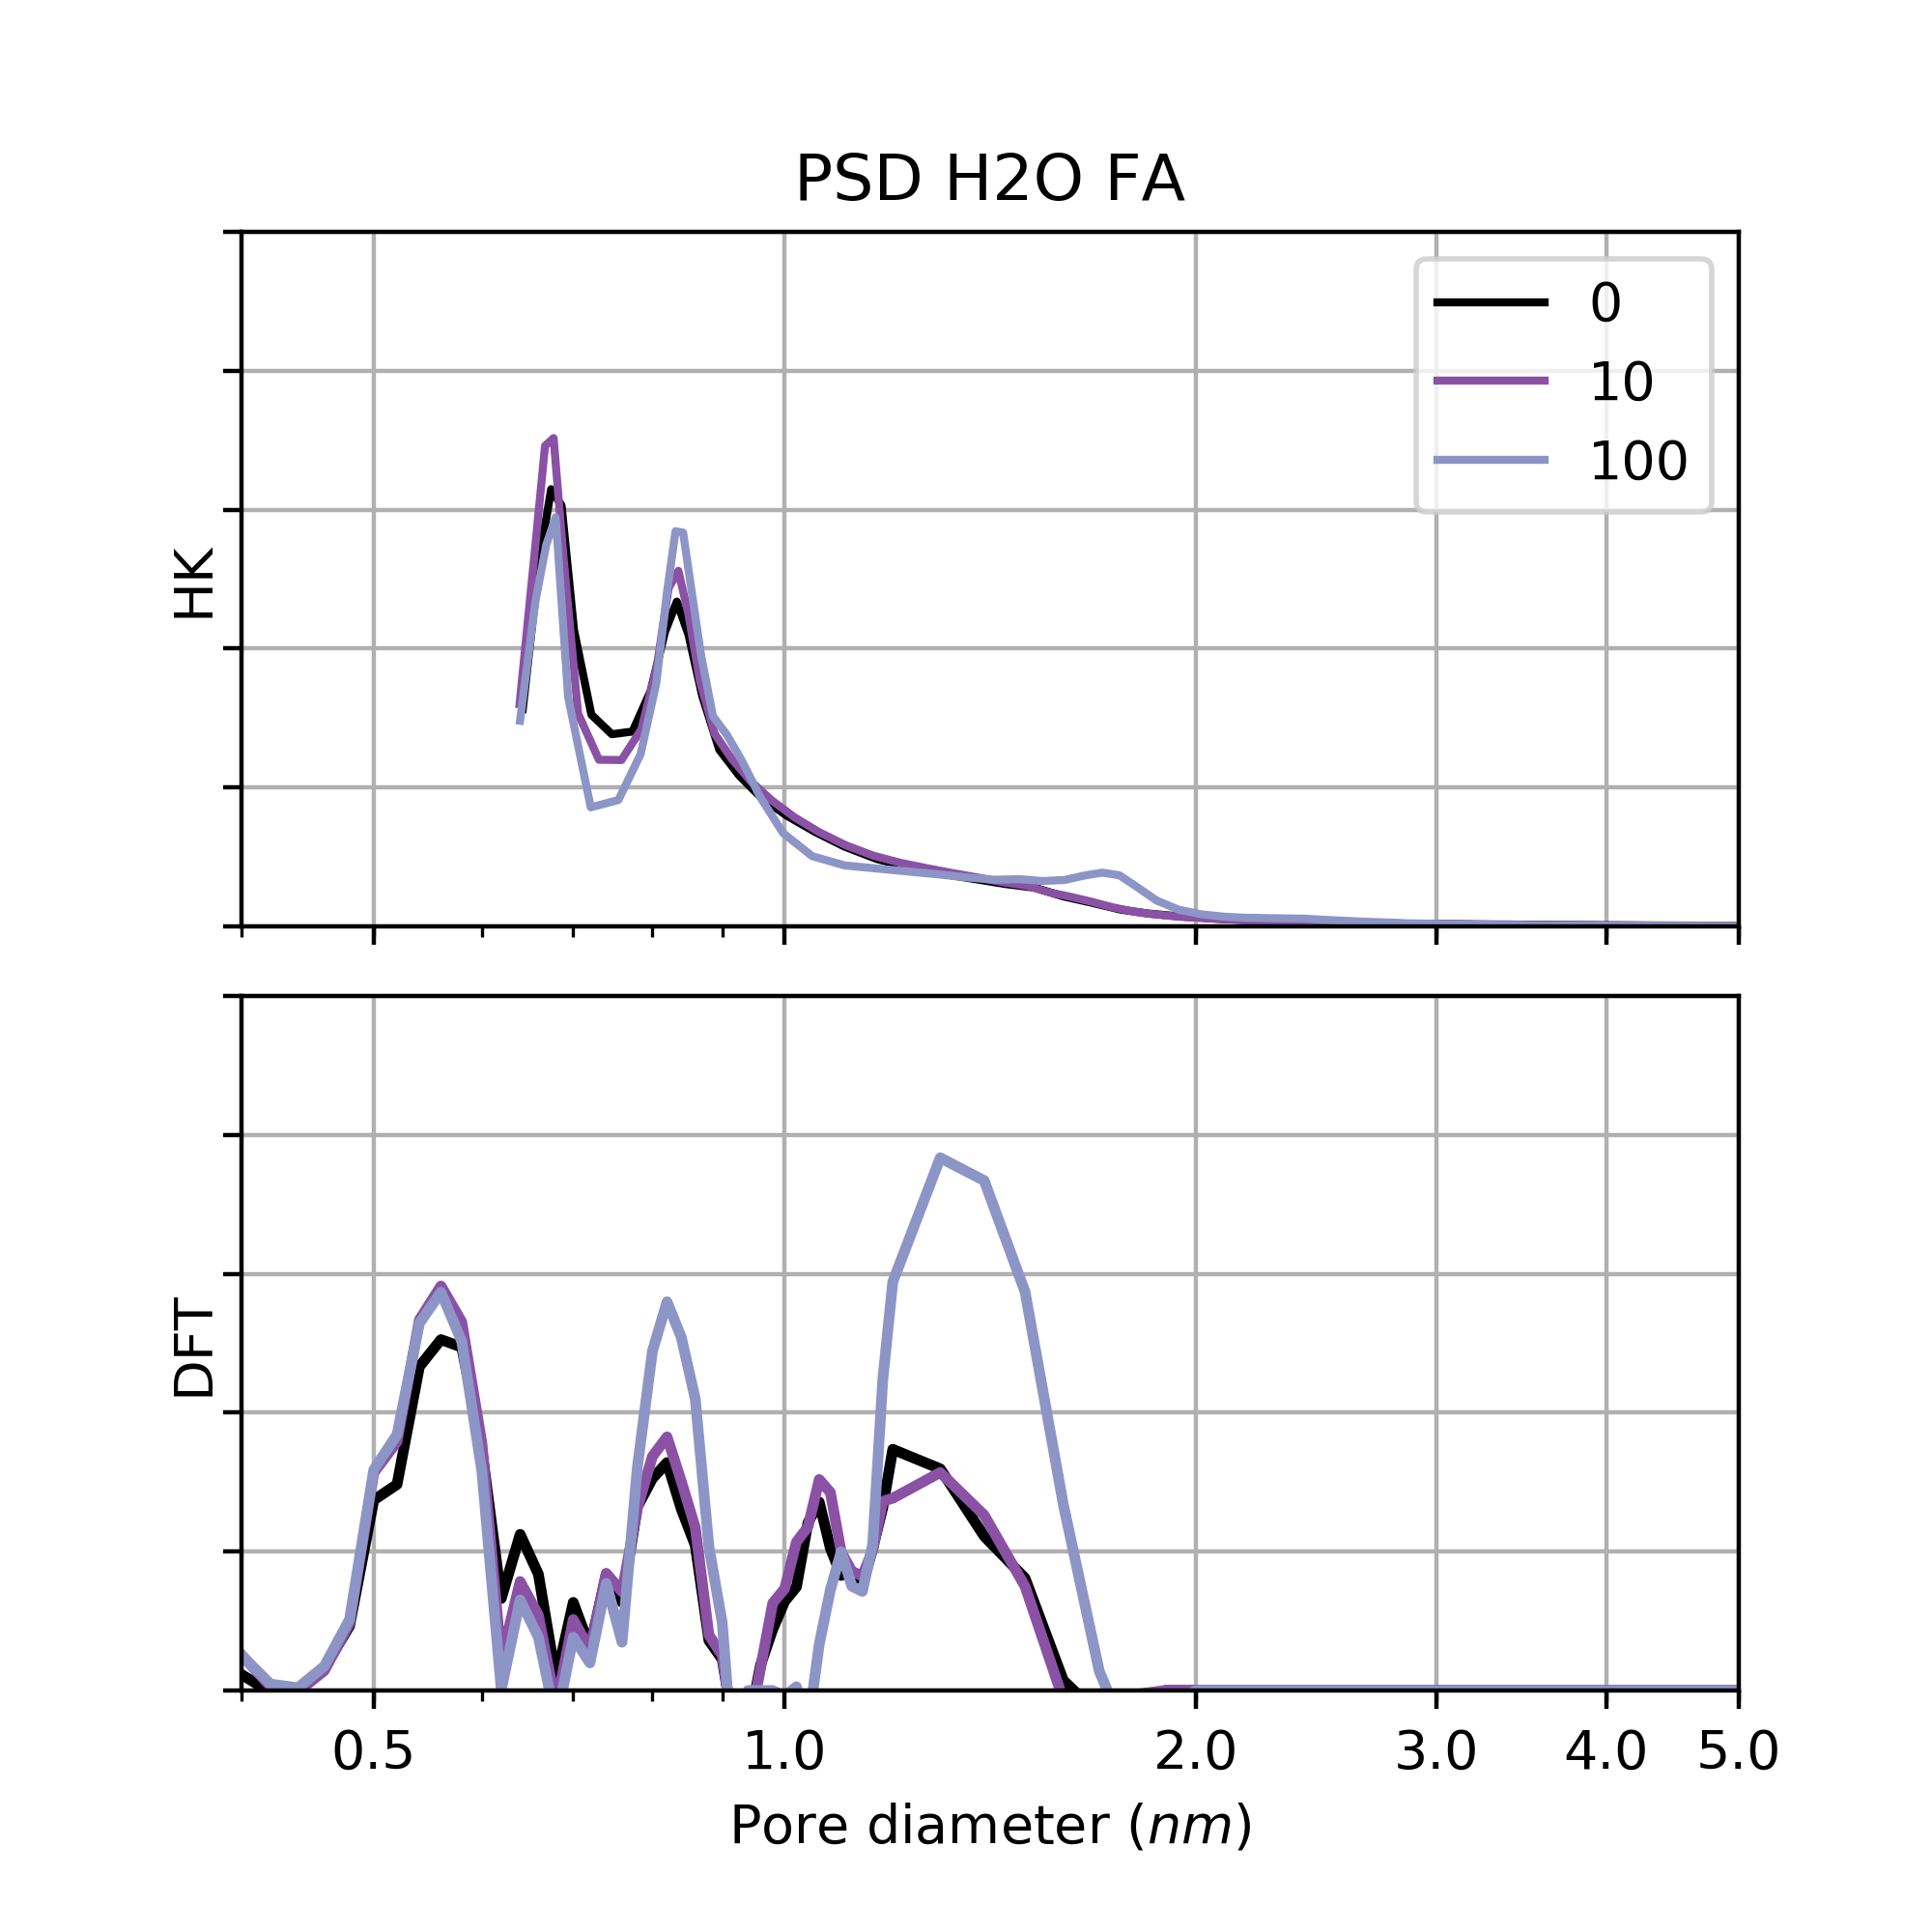
\includegraphics[width=\textwidth]{n2phys/h2o-fa-psd}%
        \label{appx:def:fig:psd-h2o-fa}
    \end{subfigure}%
    \begin{subfigure}{0.25\linewidth}
        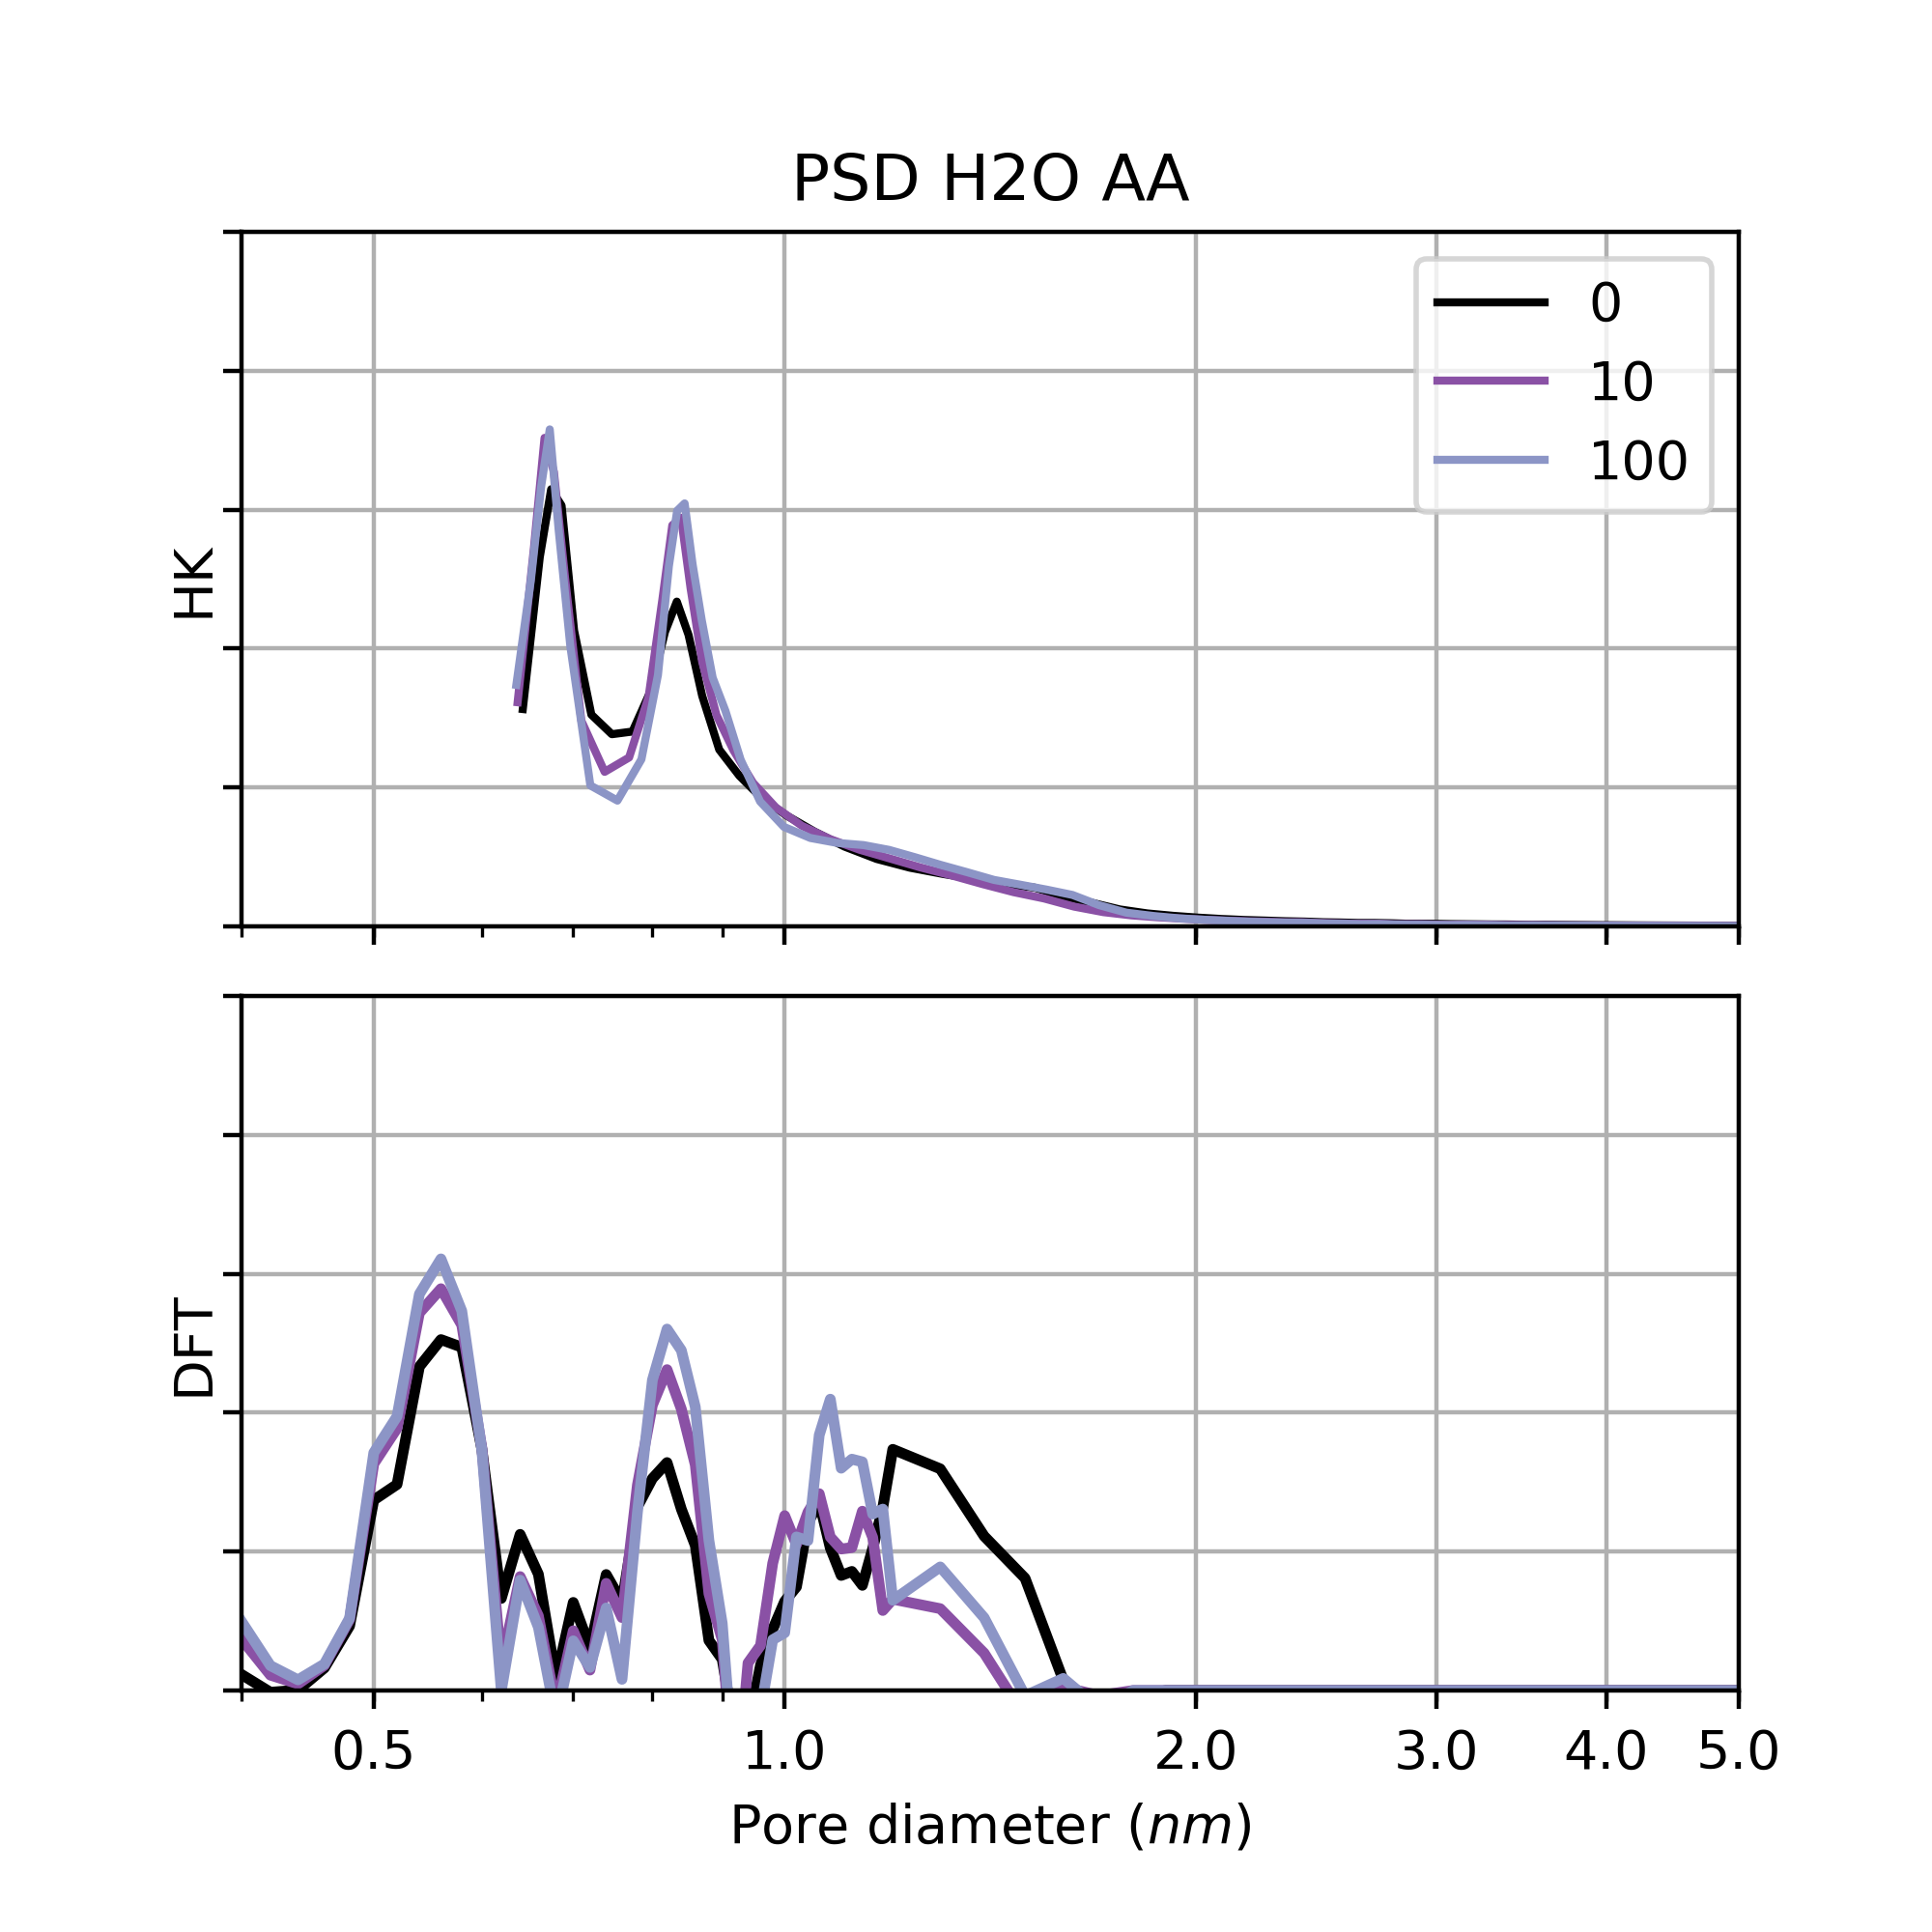
\includegraphics[width=\textwidth]{n2phys/h2o-aa-psd}%
        \label{appx:def:fig:psd-h2o-aa}
    \end{subfigure}%
    \begin{subfigure}{0.25\linewidth}
        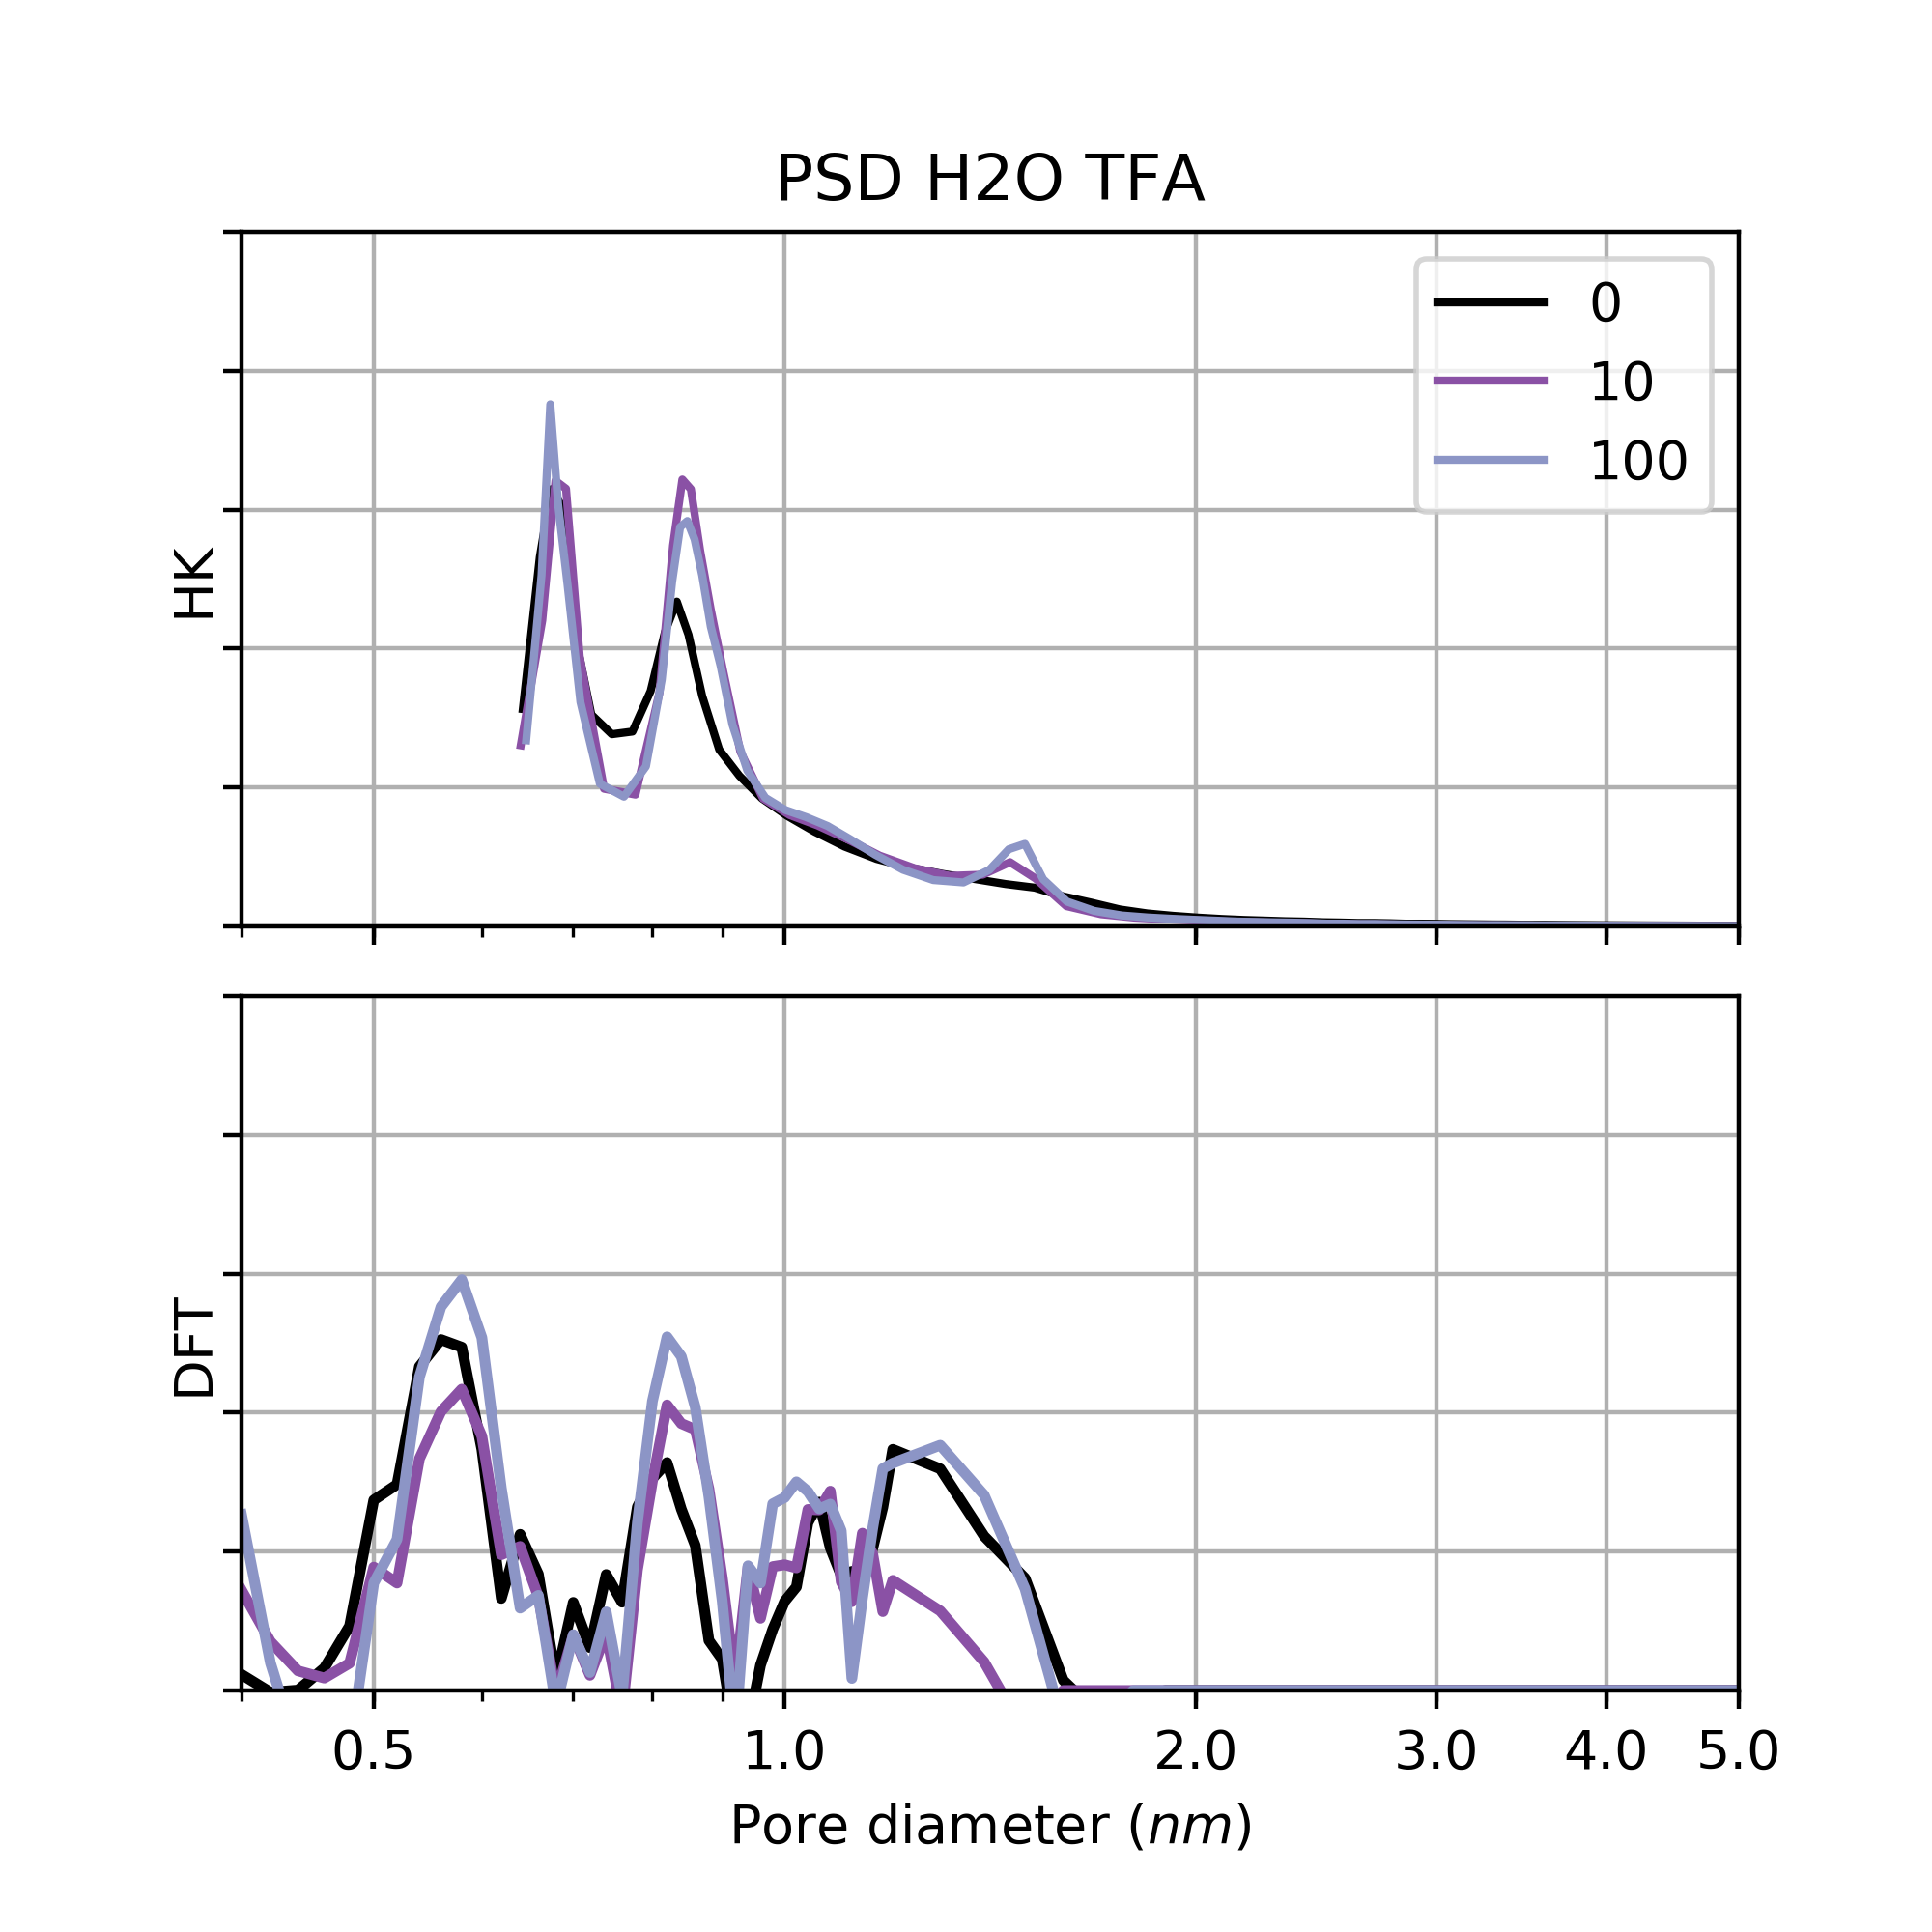
\includegraphics[width=\textwidth]{n2phys/h2o-tfa-psd}%
        \label{appx:def:fig:psd-h2o-tfa}
    \end{subfigure}%
    
    \begin{subfigure}{0.25\linewidth}
        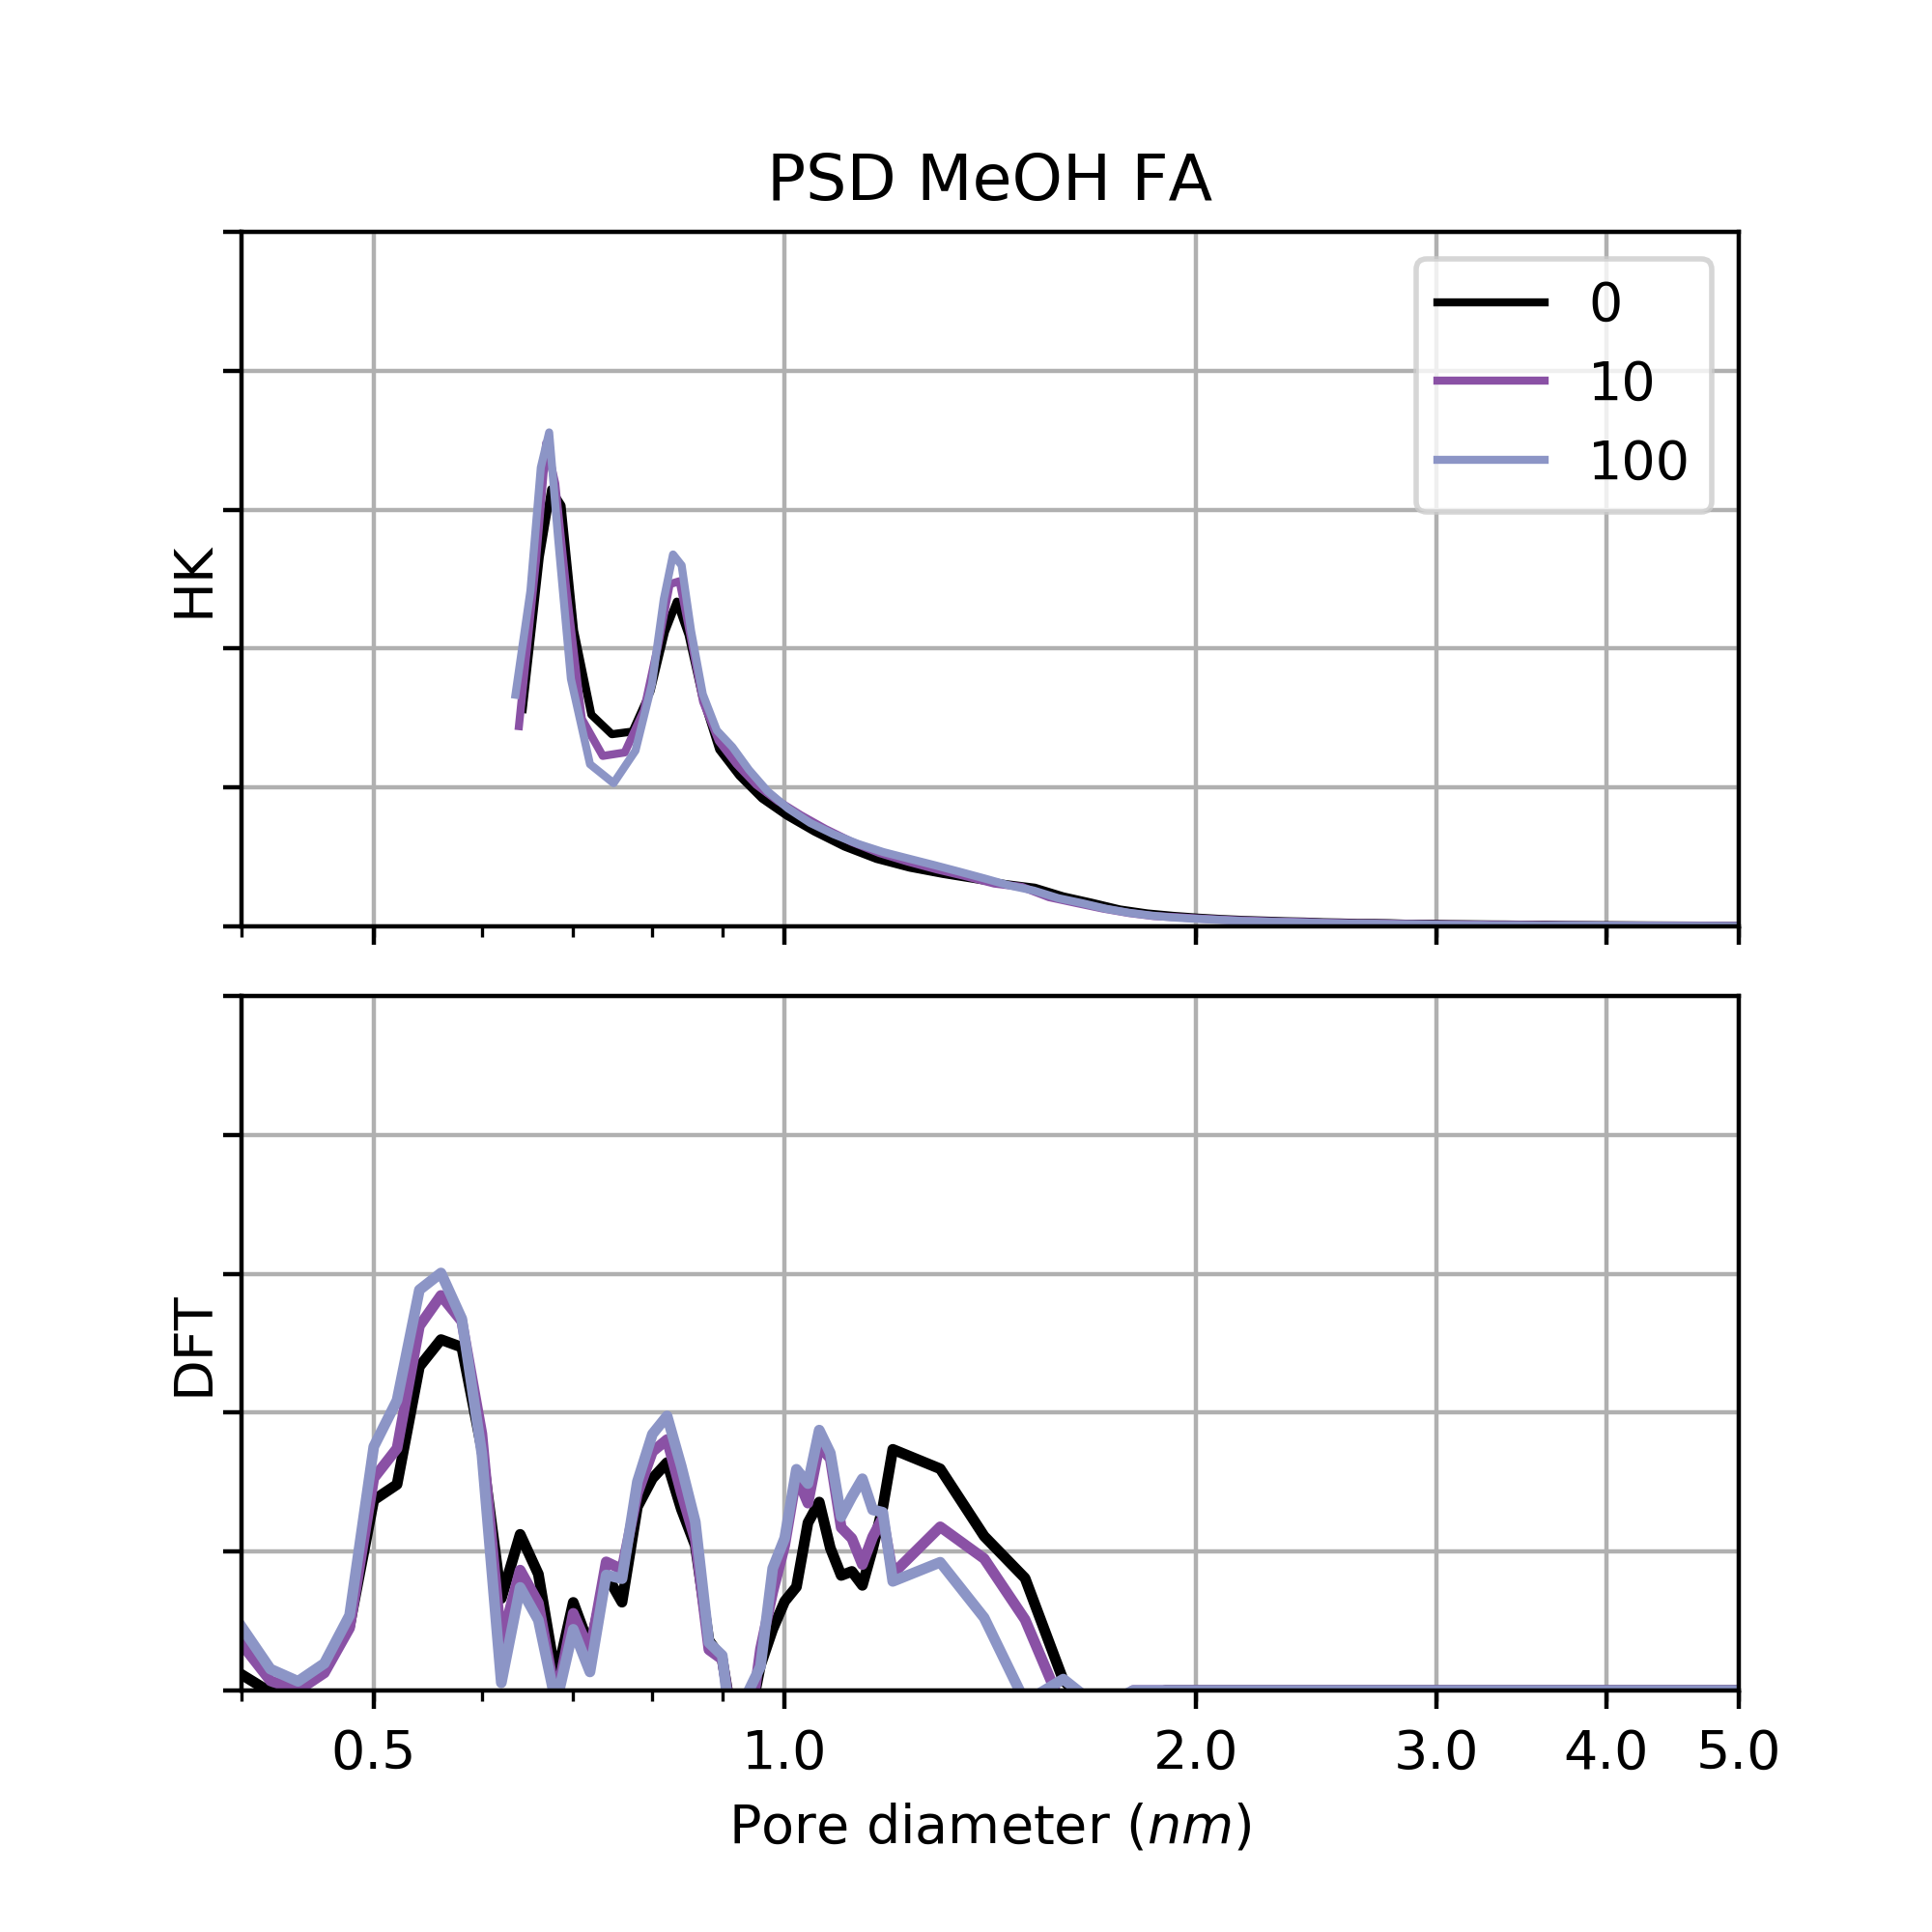
\includegraphics[width=\textwidth]{n2phys/meoh-fa-psd}%
        \label{appx:def:fig:psd-meoh-fa}
    \end{subfigure}%
    \begin{subfigure}{0.25\linewidth}
        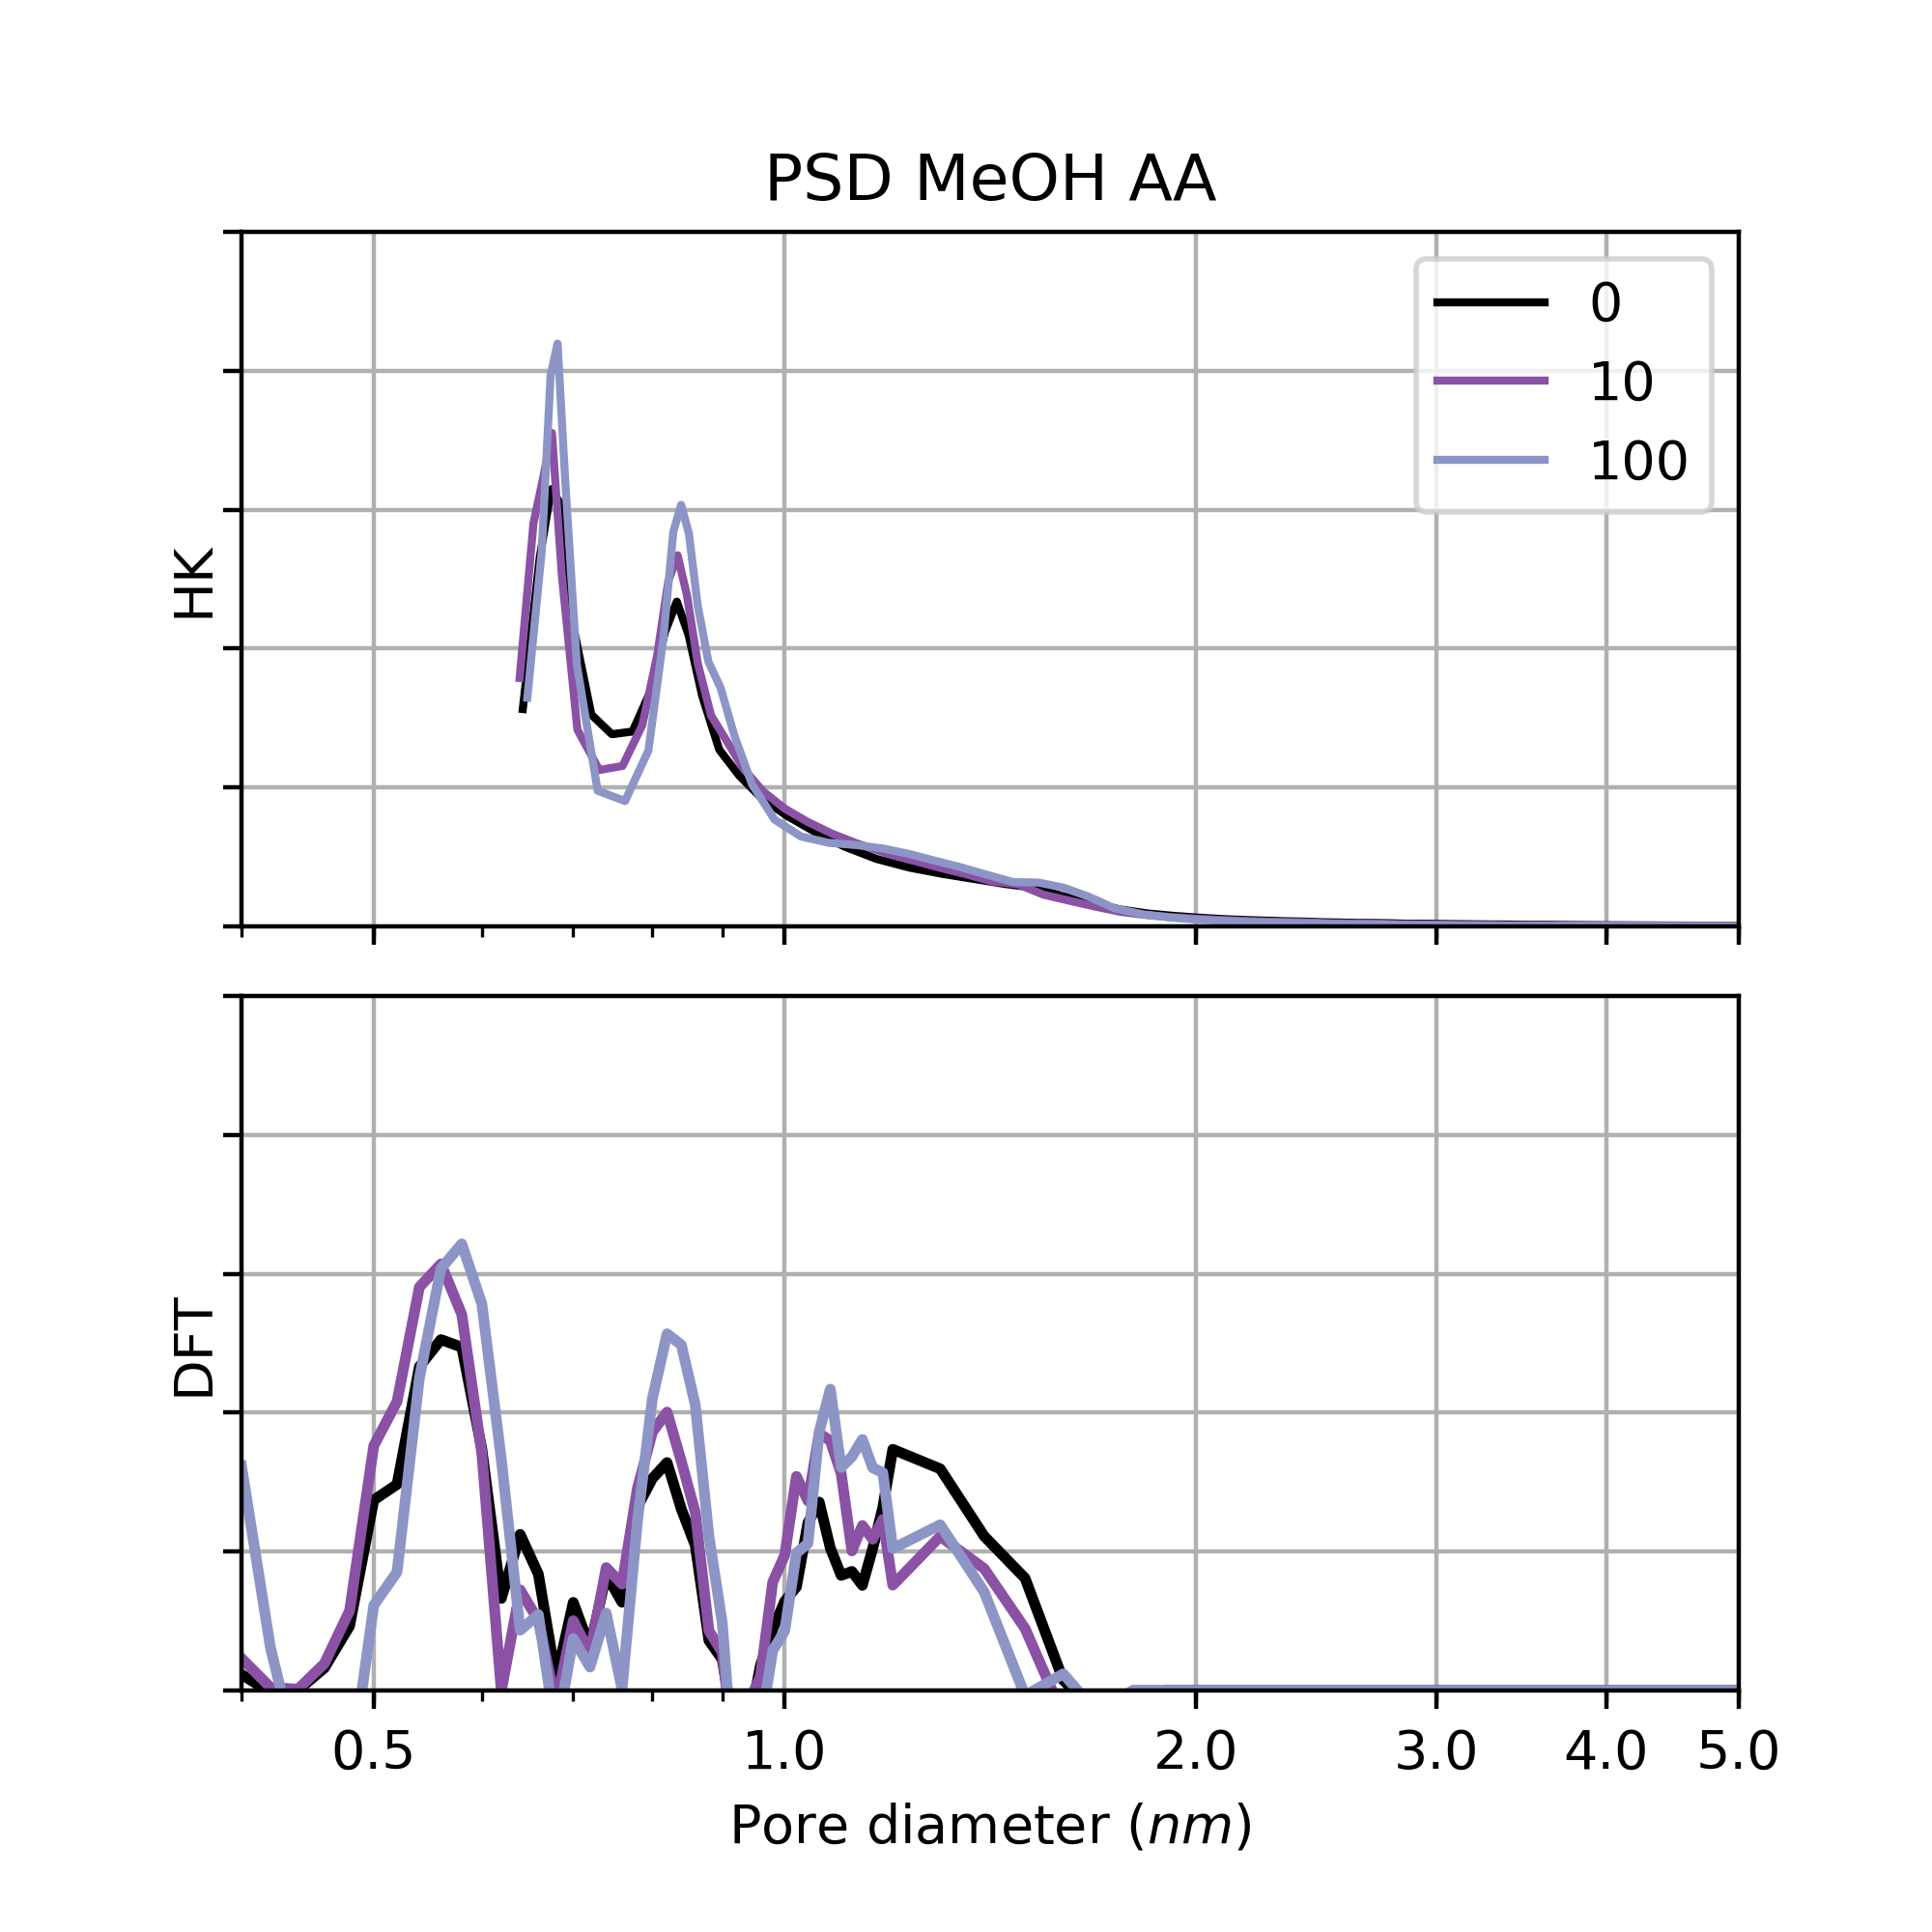
\includegraphics[width=\textwidth]{n2phys/meoh-aa-psd}%
        \label{appx:def:fig:psd-meoh-aa}
    \end{subfigure}%
    \begin{subfigure}{0.25\linewidth}
        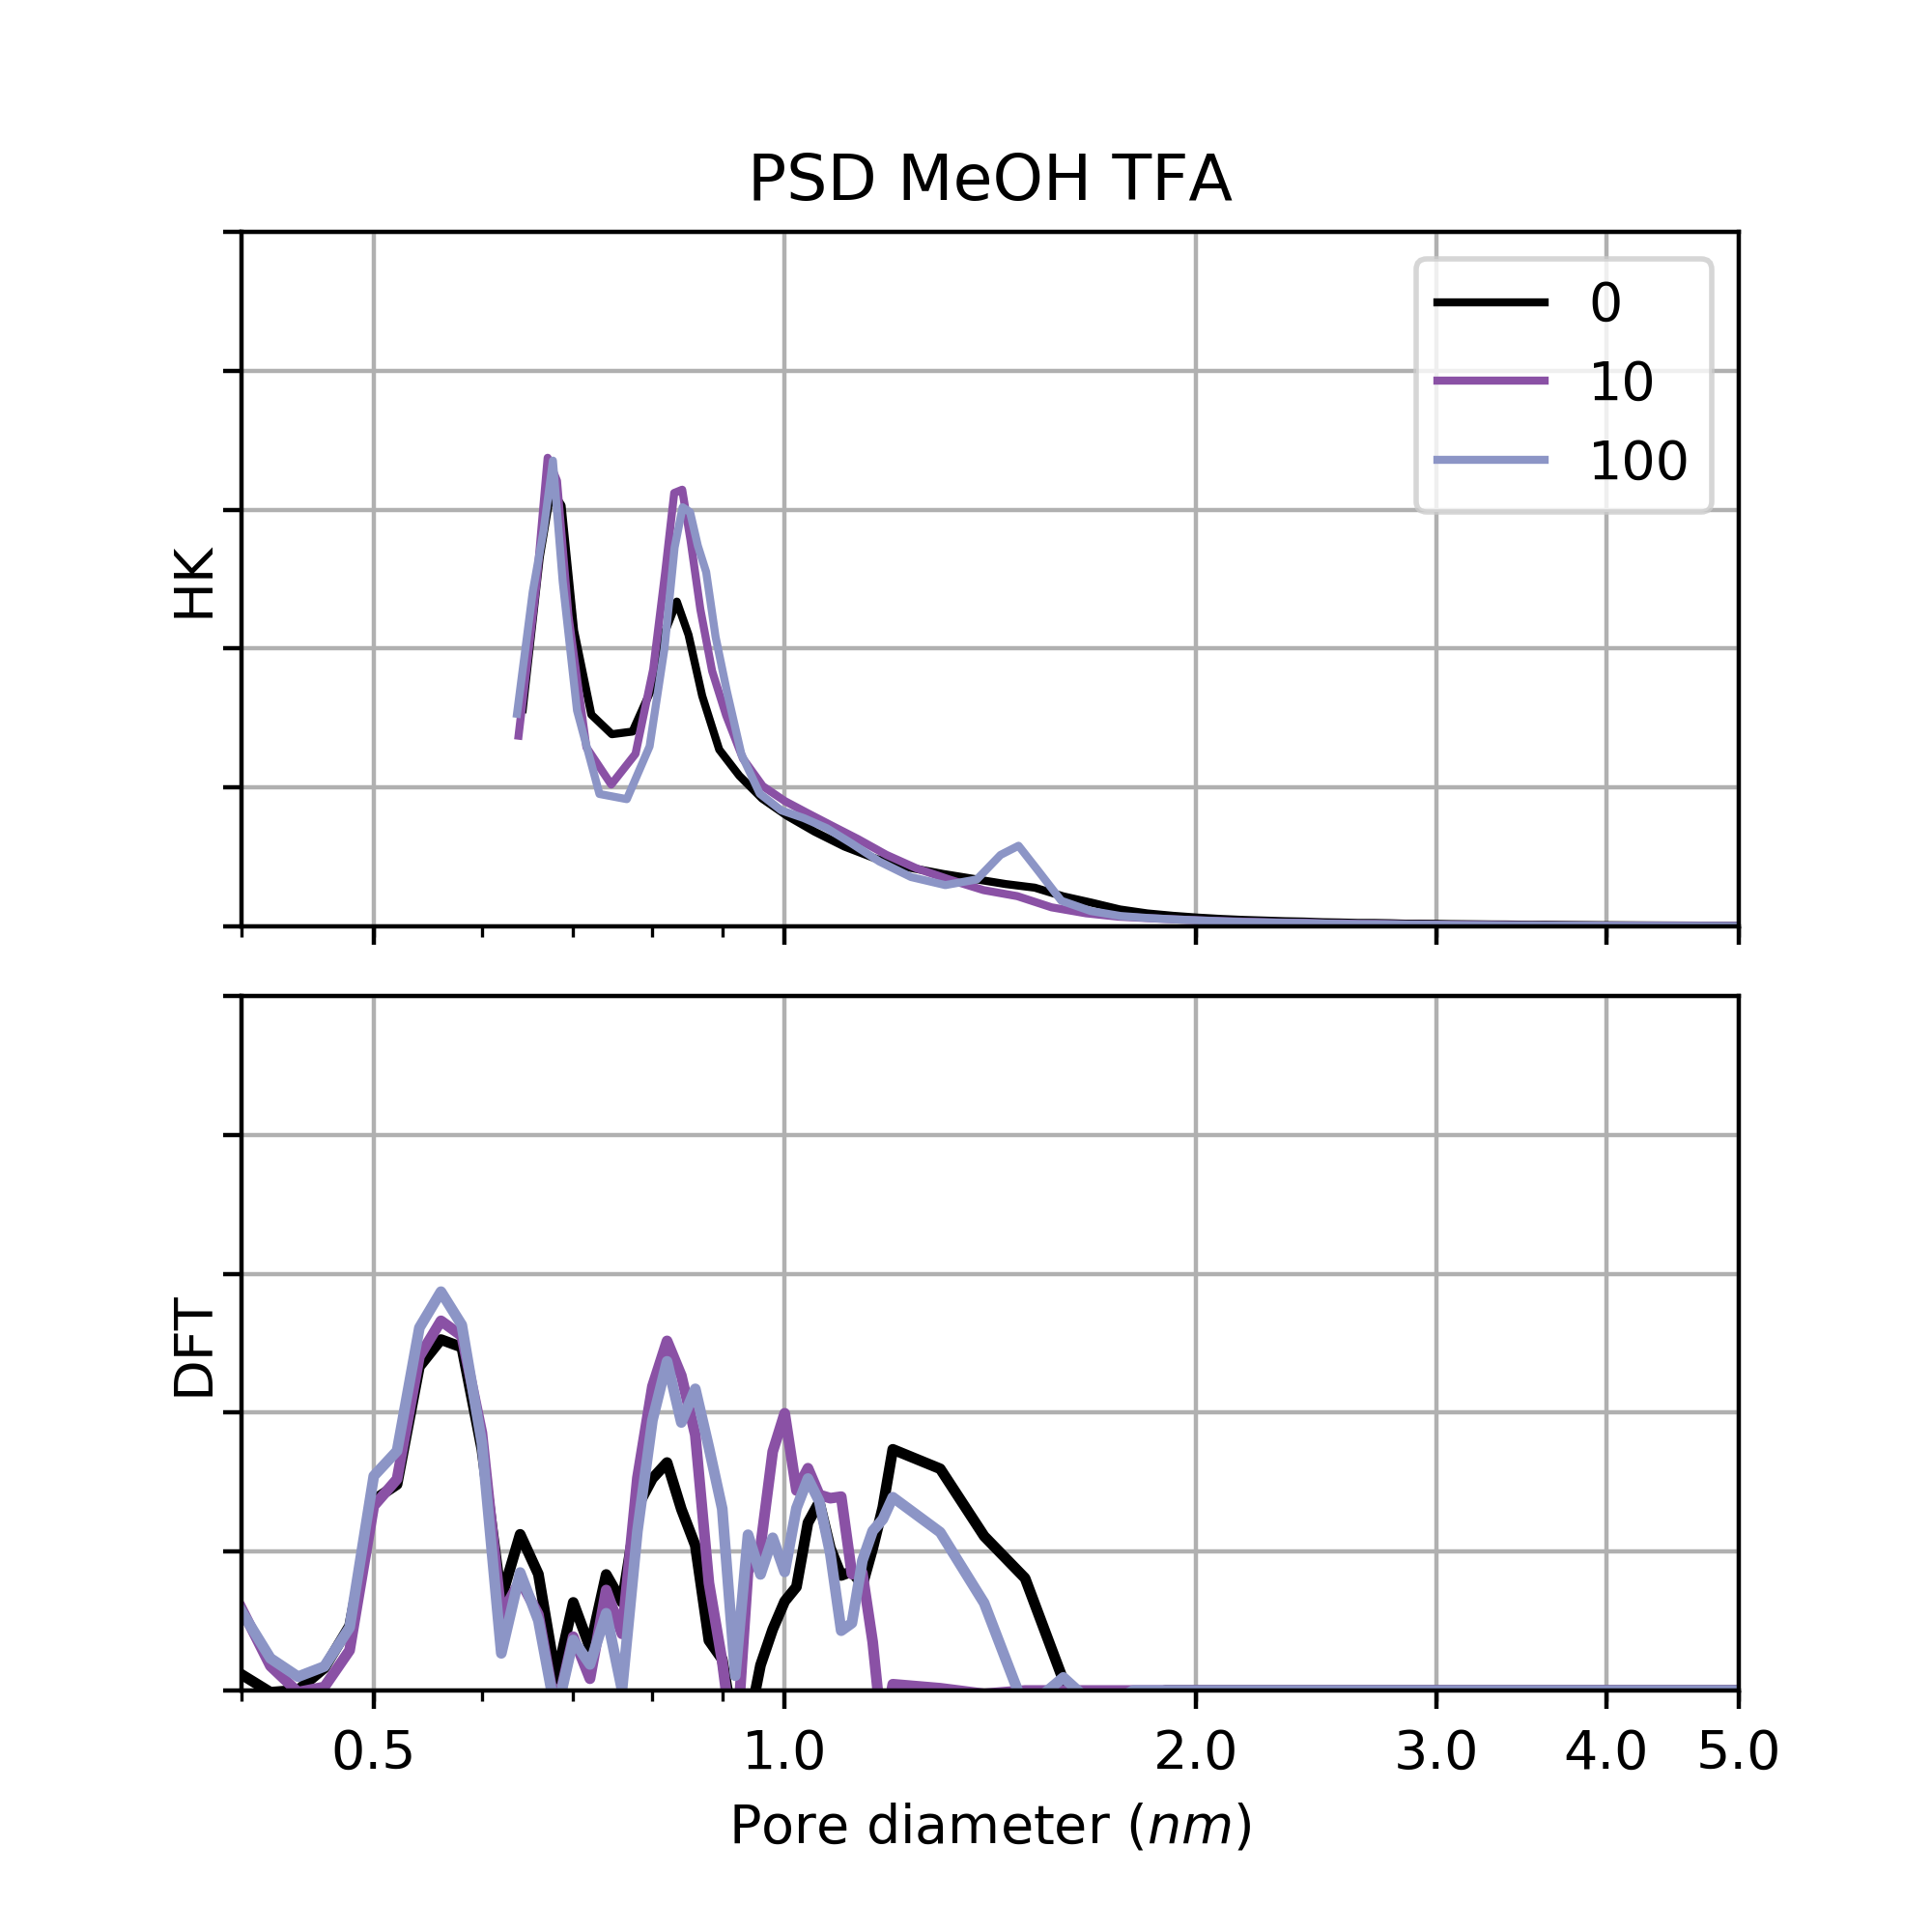
\includegraphics[width=\textwidth]{n2phys/meoh-tfa-psd}%
        \label{appx:def:fig:psd-meoh-tfa}
    \end{subfigure}%
    \begin{subfigure}{0.25\linewidth}
        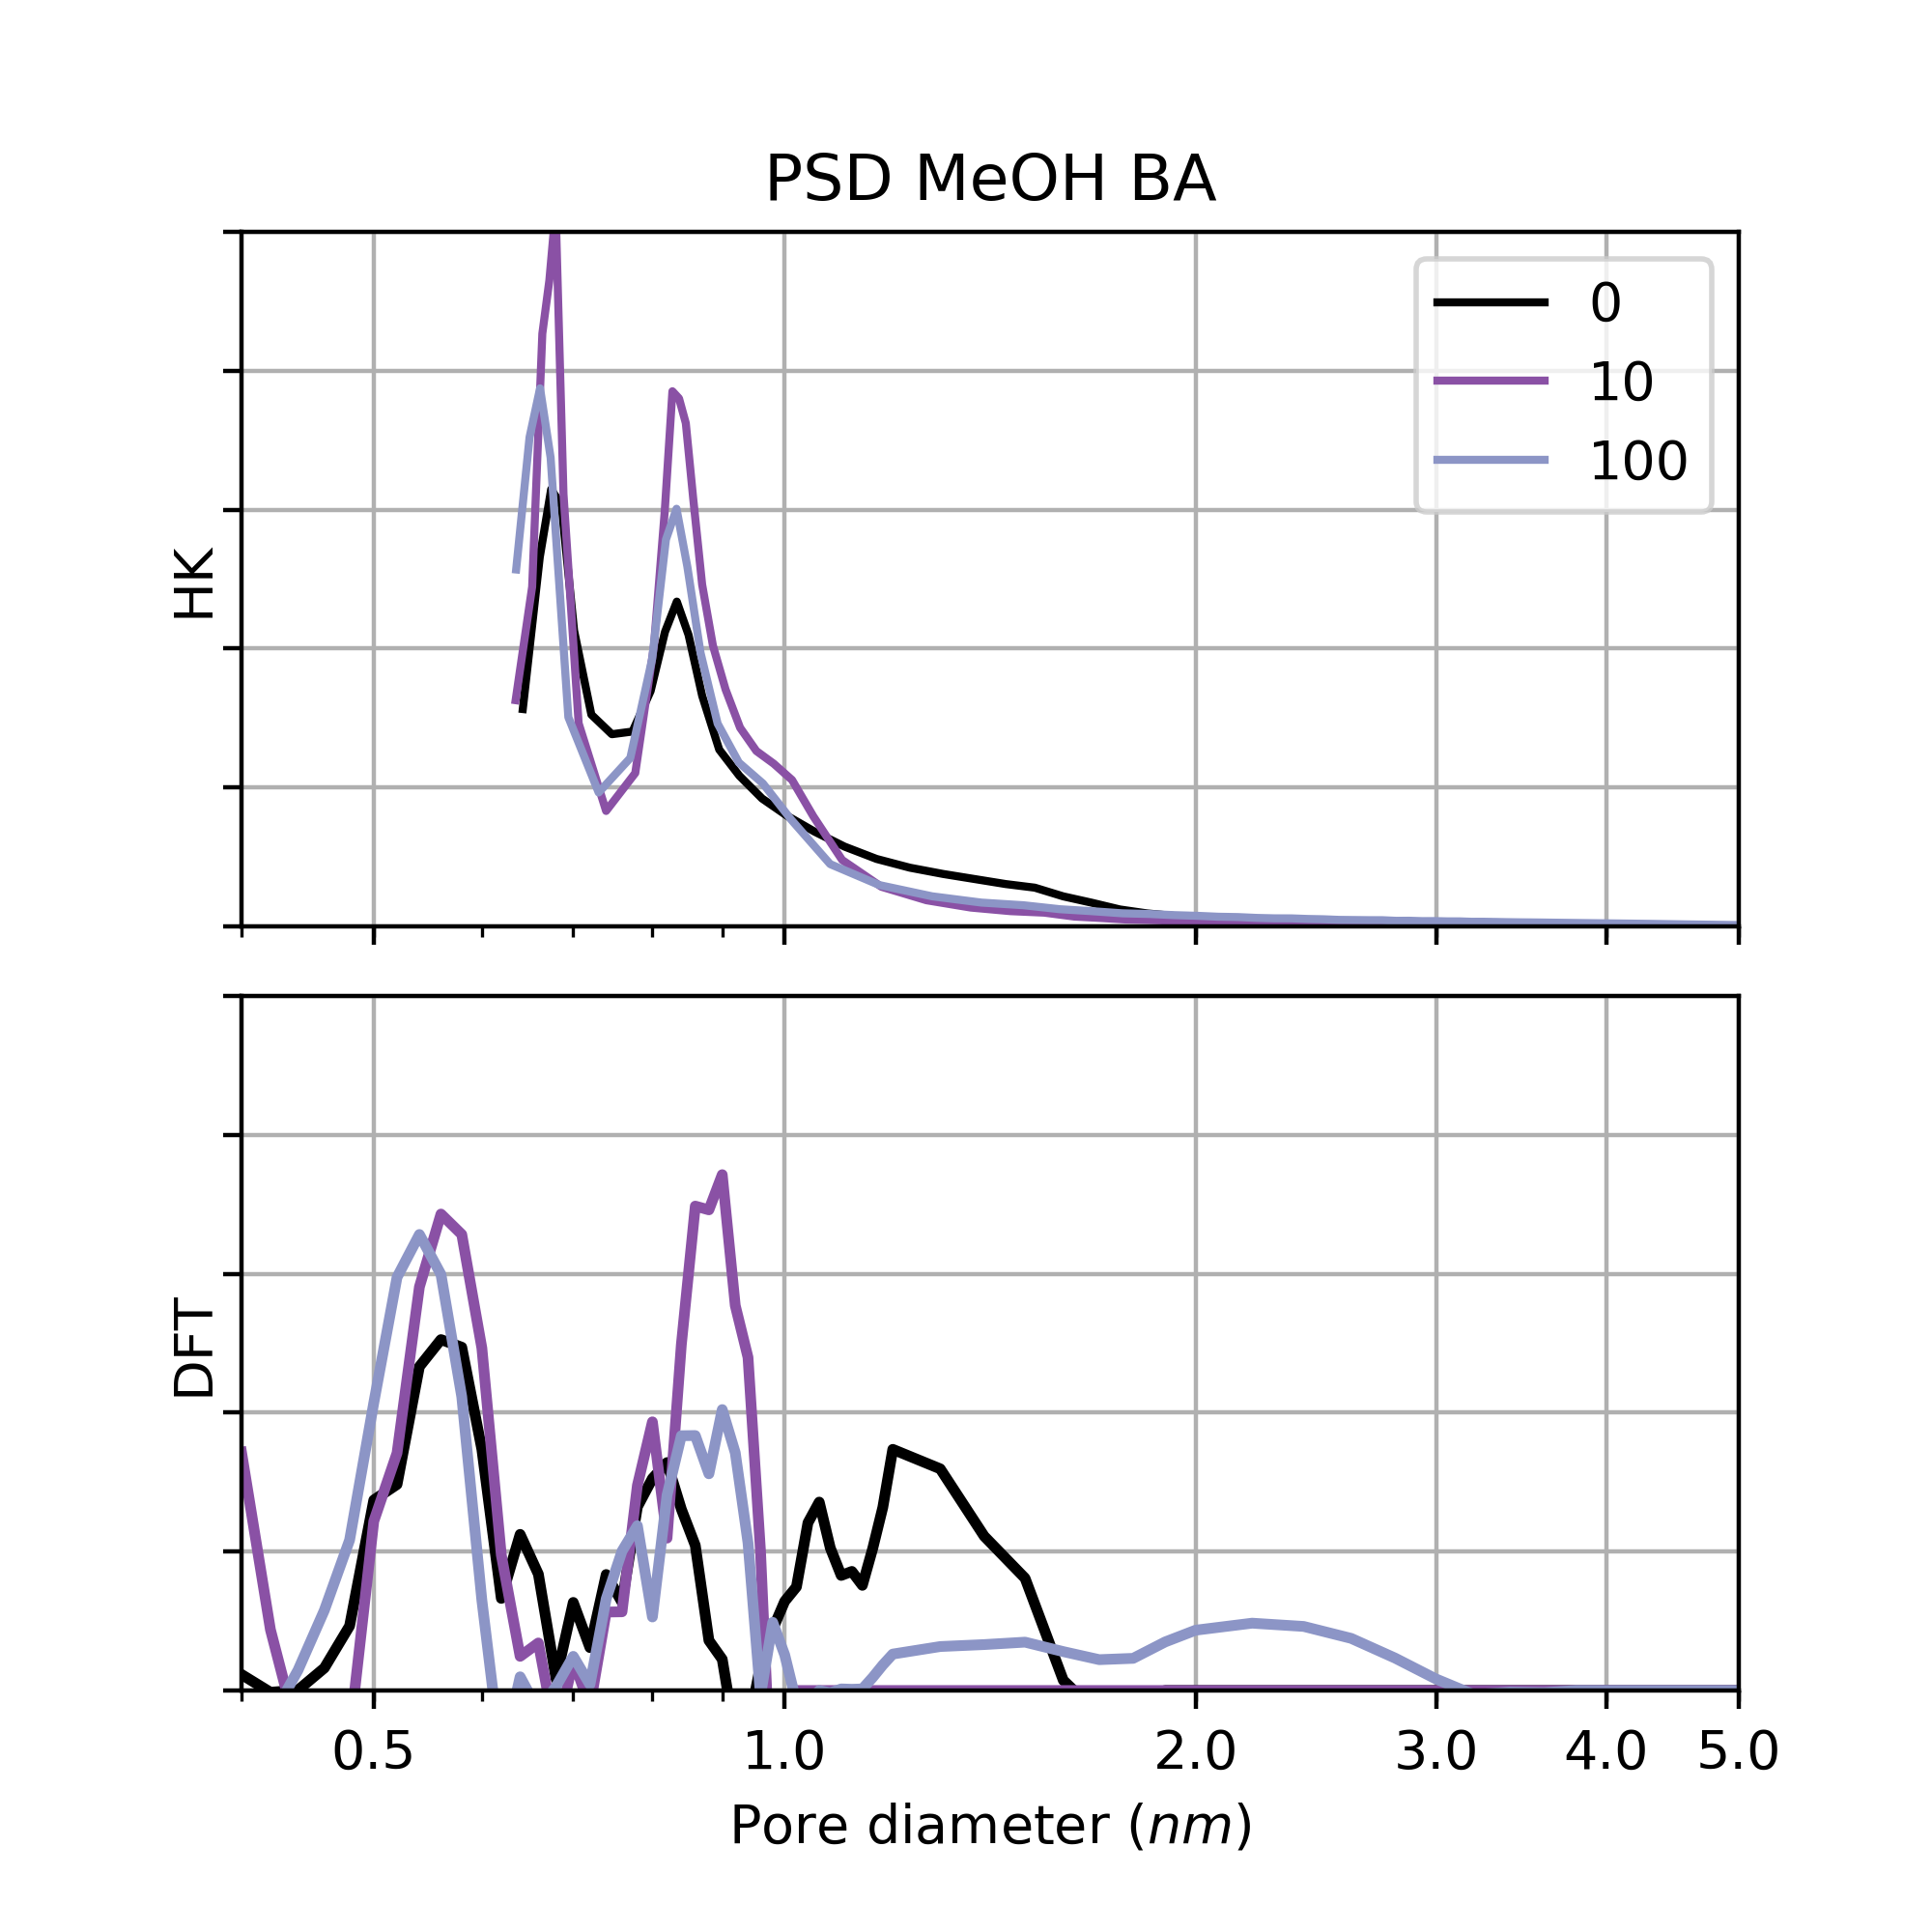
\includegraphics[width=\textwidth]{n2phys/meoh-ba-psd}%
        \label{appx:def:fig:psd-meoh-ba}
    \end{subfigure}%
    
    \begin{subfigure}{0.25\linewidth}
        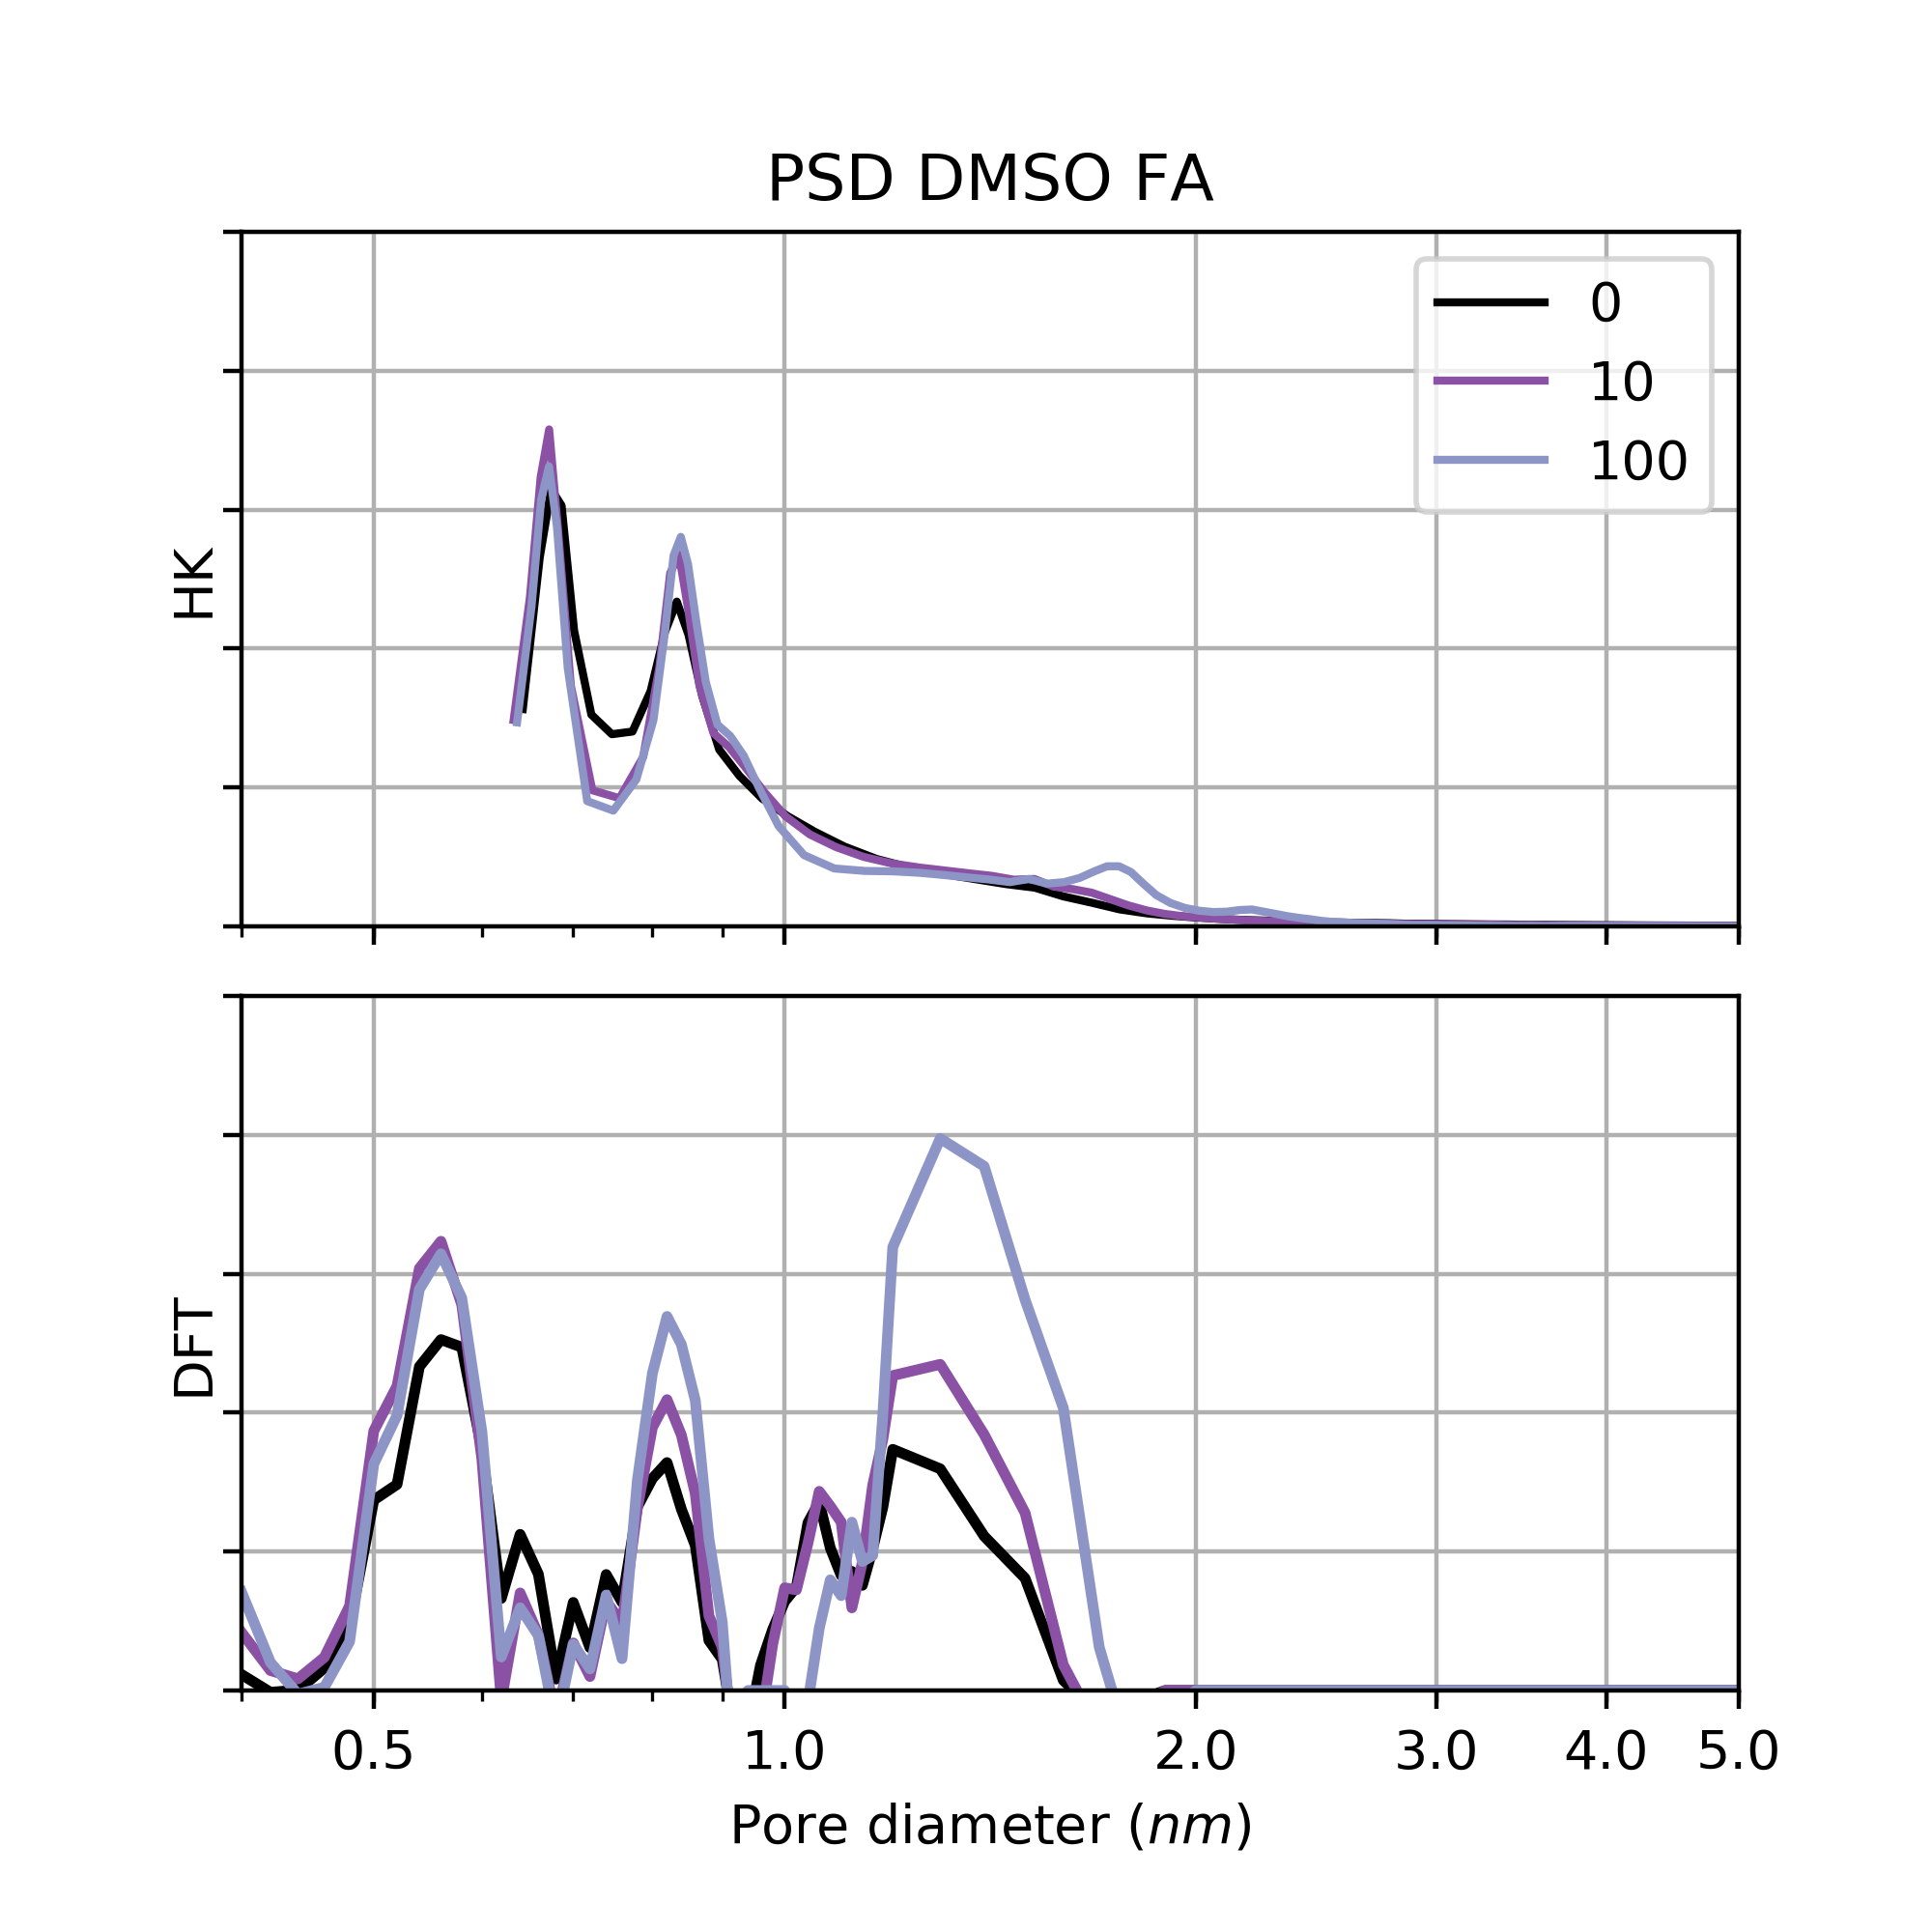
\includegraphics[width=\textwidth]{n2phys/dmso-fa-psd}%
        \label{appx:def:fig:psd-dmso-fa}
    \end{subfigure}%
    \begin{subfigure}{0.25\linewidth}
        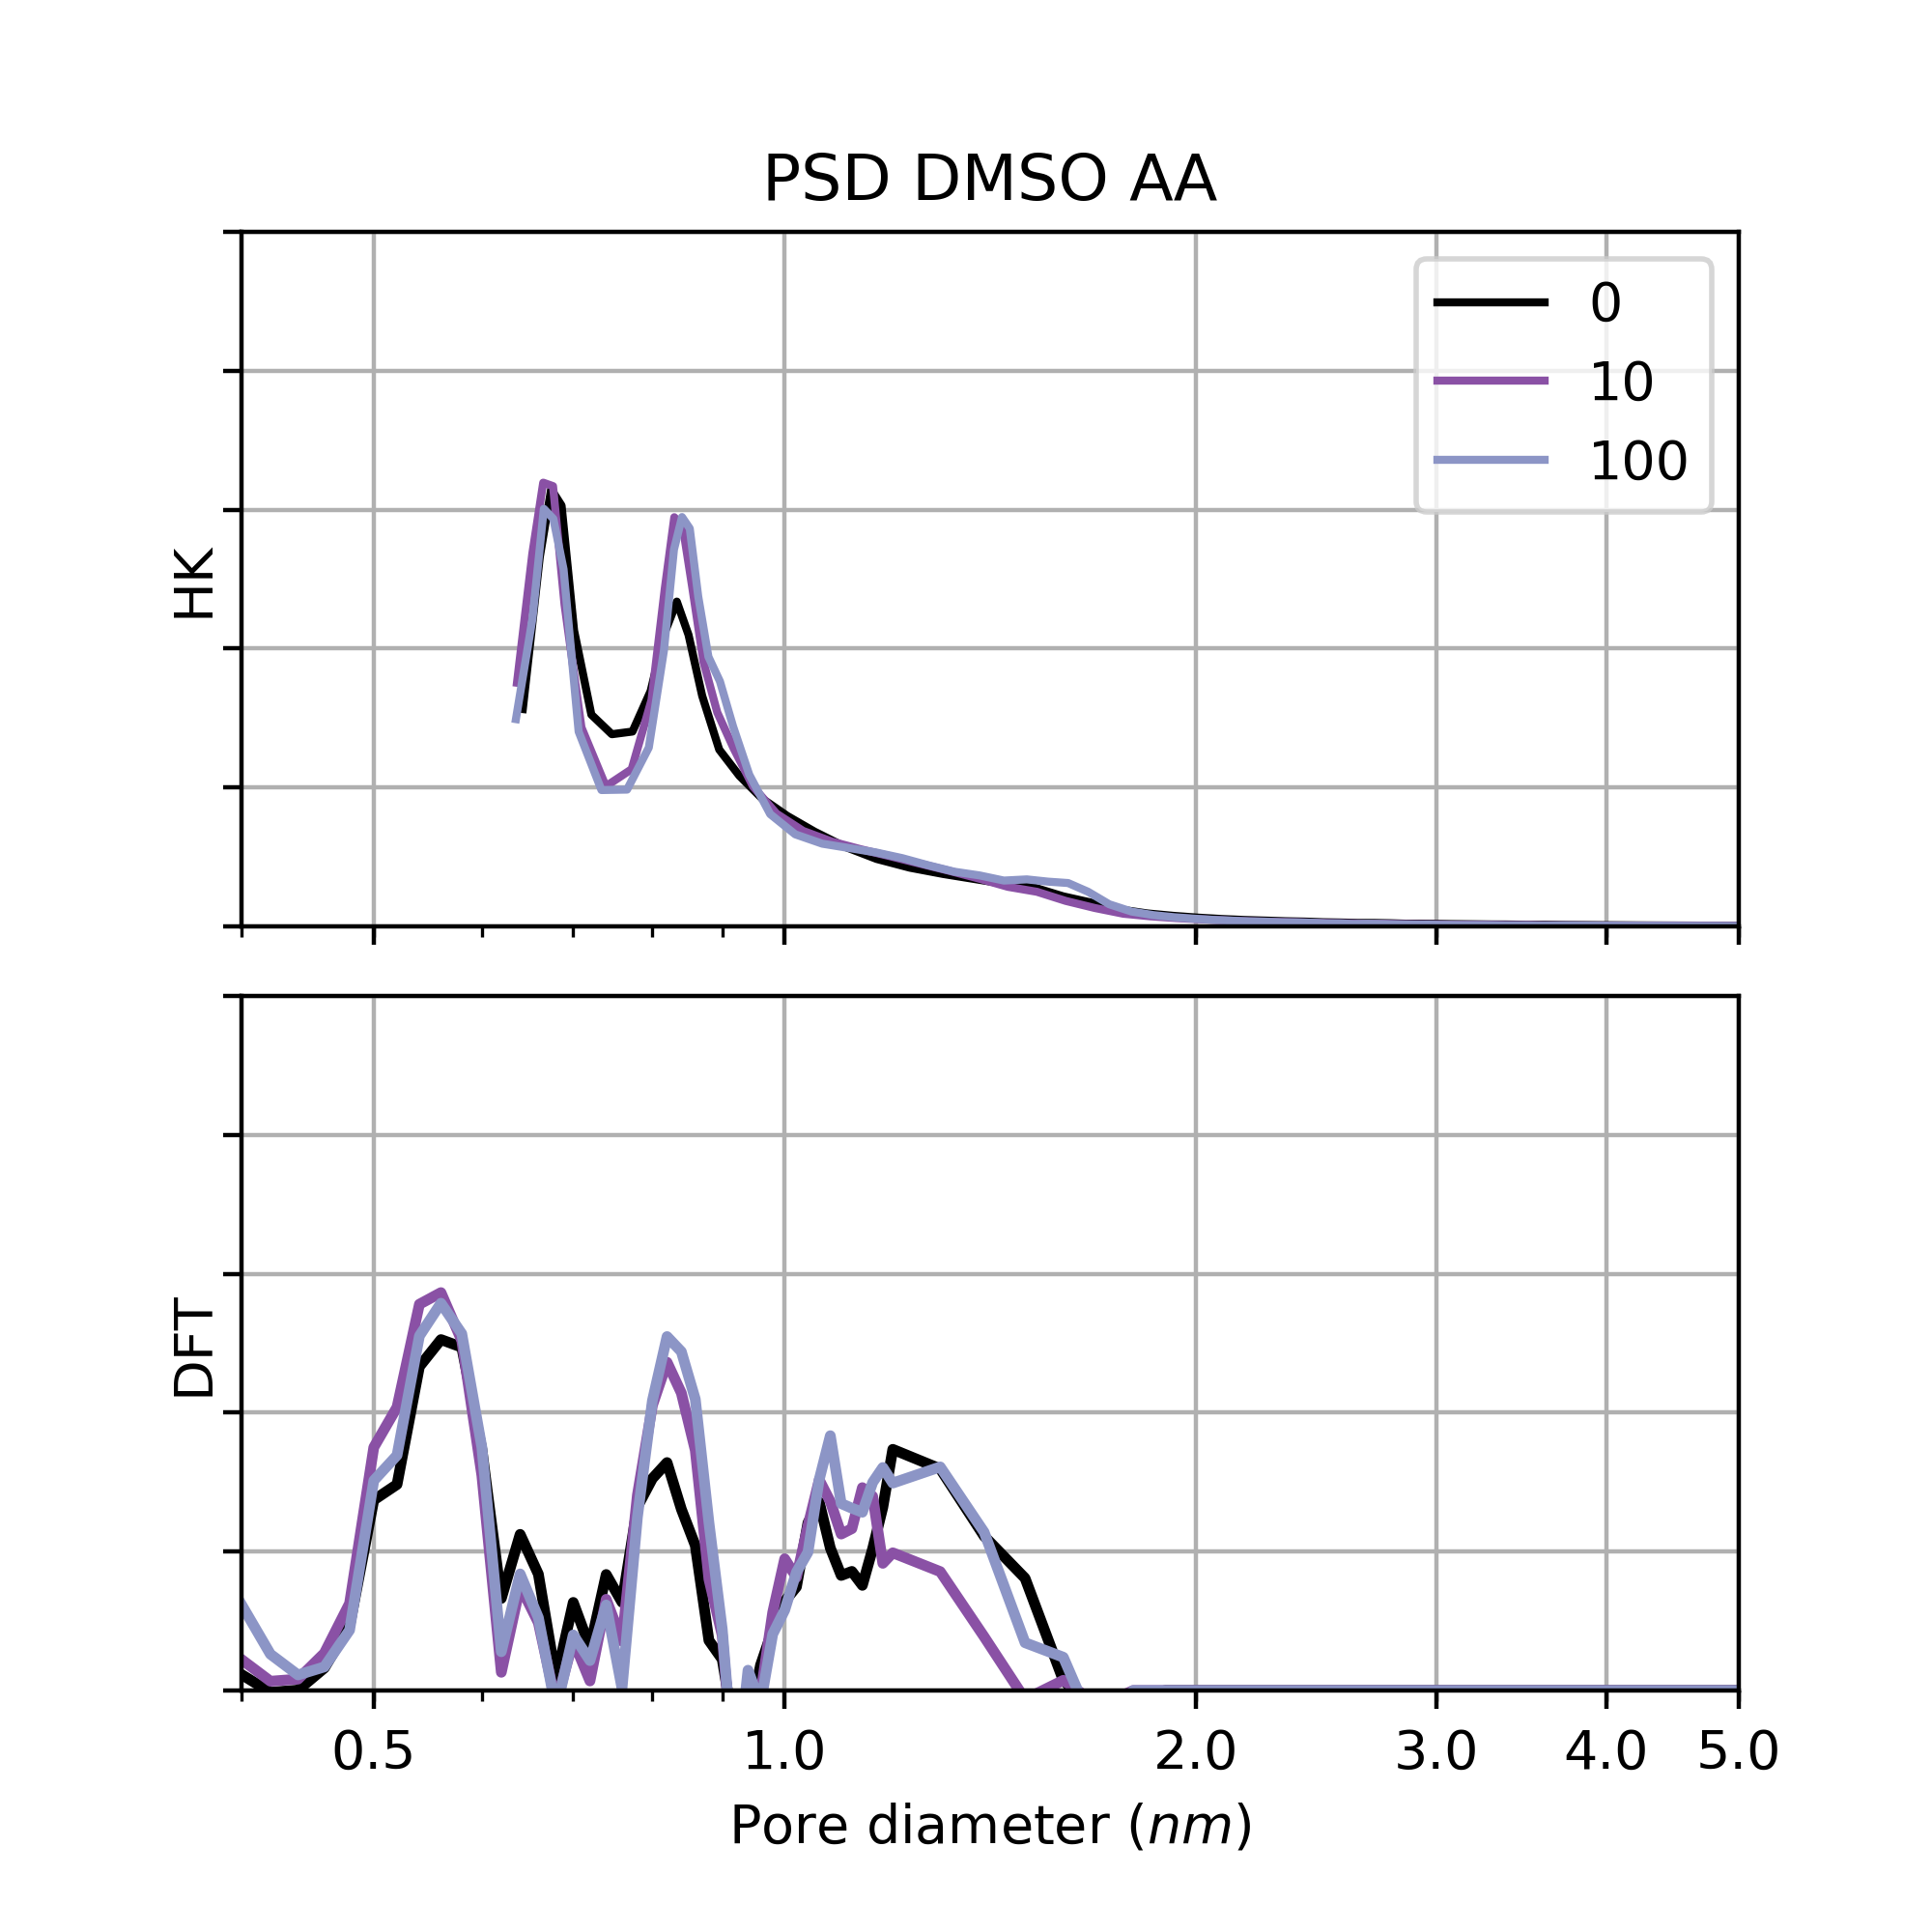
\includegraphics[width=\textwidth]{n2phys/dmso-aa-psd}%
        \label{appx:def:fig:psd-dmso-aa}
    \end{subfigure}%
    \begin{subfigure}{0.25\linewidth}
        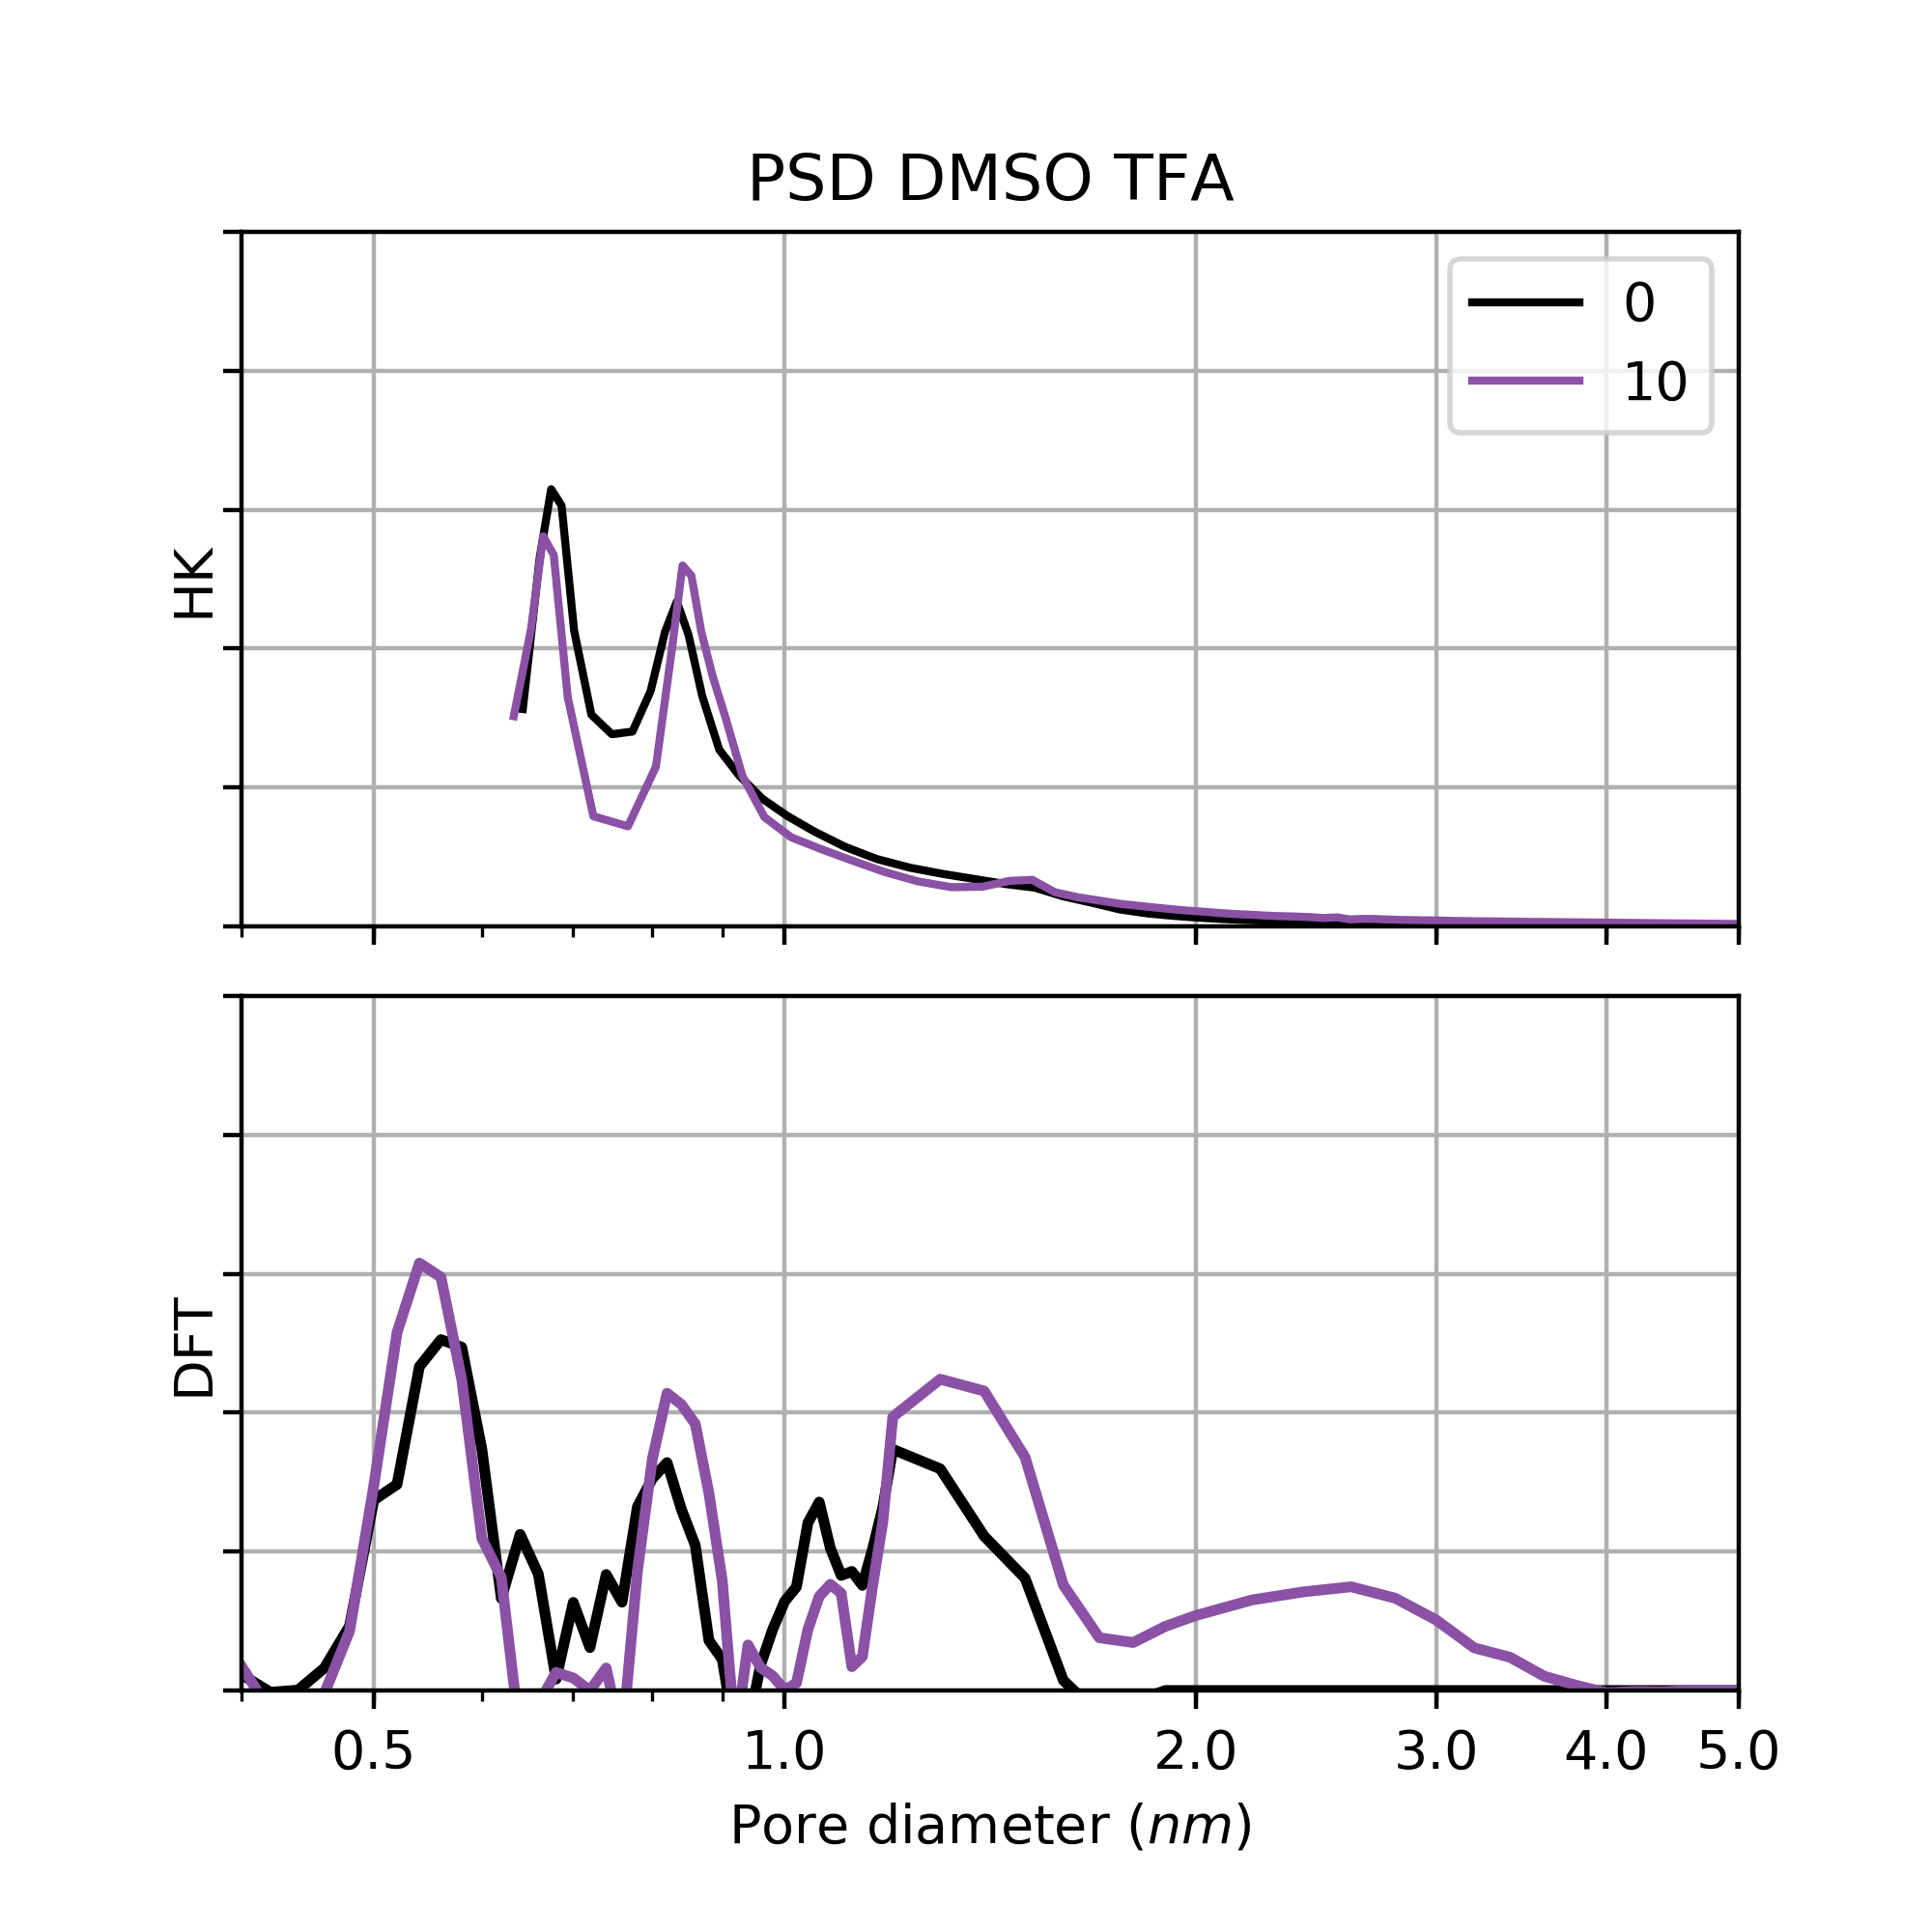
\includegraphics[width=\textwidth]{n2phys/dmso-tfa-psd}%
        \label{appx:def:fig:psd-dmso-tfa}
    \end{subfigure}%
    \begin{subfigure}{0.25\linewidth}
        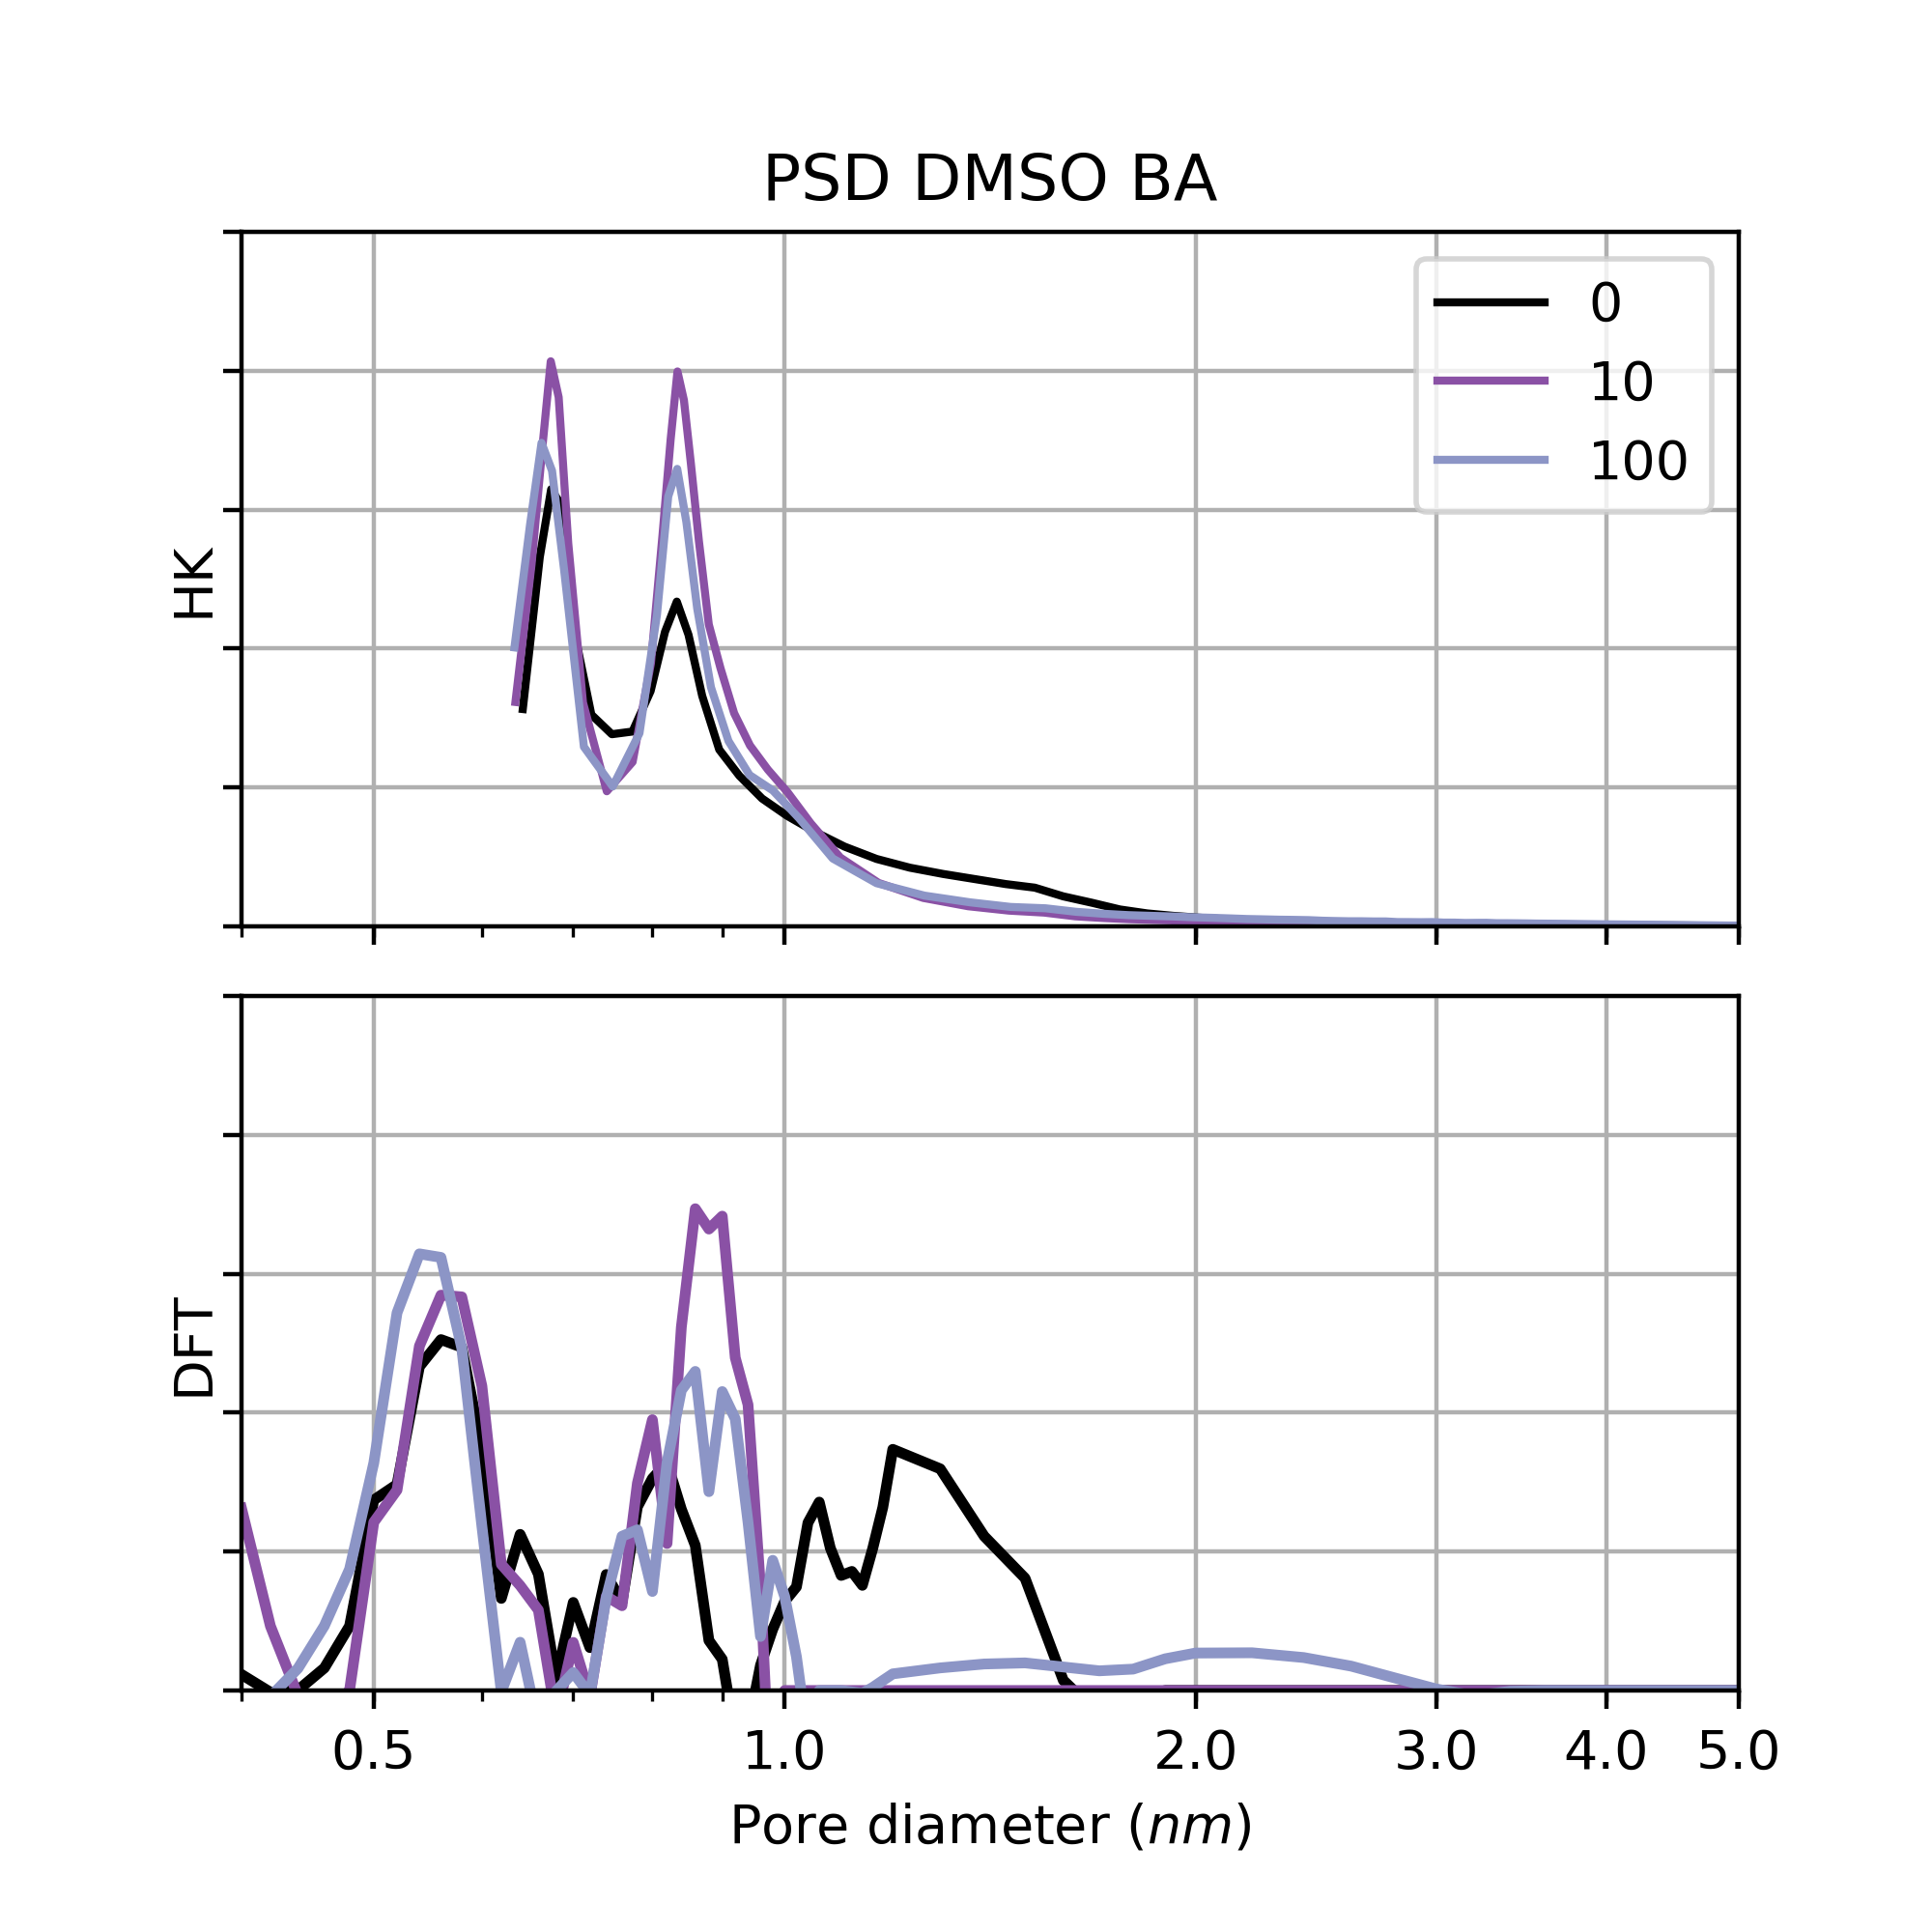
\includegraphics[width=\textwidth]{n2phys/dmso-ba-psd}%
        \label{appx:def:fig:psd-dmso-ba}
    \end{subfigure}%

\end{figure}
